% ===================================================================
% MAIN FILE
% COMPILE WITH: XeLaTeX
% ===================================================================

\documentclass[10pt, a4paper]{report}


%---------- PACKAGES ----------
\usepackage[utf8]{inputenc}
\usepackage[T1]{fontenc}
\usepackage[margin=1in]{geometry}
\usepackage{graphicx}
\usepackage{tabularx}
\usepackage{ragged2e}
\usepackage{booktabs}
\usepackage{caption}
\usepackage{array}
\usepackage{siunitx}
\usepackage{amsmath}
\usepackage[hidelinks]{hyperref}

\DeclareSIUnit{\fps}{frames~per~second}

\makeatletter
\newcommand\frontmatter{%
    \cleardoublepage
    \pagenumbering{roman}}
\newcommand\mainmatter{%
    \cleardoublepage
    \pagenumbering{arabic}}
\newcommand\backmatter{%
  \if@openright
    \cleardoublepage
  \else
    \clearpage
  \fi
}
\makeatother



\begin{document}
\frontmatter

%---------- TITLE PAGE ----------
\begin{titlepage}
    \centering 
    \begin{minipage}[t]{1\textwidth}
        \raggedright 
        \large
        Syrian Arab Republic \\
        Higher Institute for Applied Sciences and Technology (HIAST) \\
        Department of Information Systems \\
        Specialization: Software Engineering and Artificial Intelligence \\
        Academic Year: 2024-2025
    \end{minipage}
    
    \vfill 
    
\includegraphics[width=3cm]{images/HIAST_logo.png} \par
    
    
    \vspace{2cm} 
    
    % Main Title
    {\huge\bfseries Monocular Depth Estimation using \par}
    {\huge\bfseries Knowledge Distillation Techniques \par}
    
    \vspace{1cm}
    
    {\Huge\bfseries Delta \par}
    
    \vfill 
    
    % Author and Supervisor information in a two-column layout
    \begin{minipage}[t]{0.4\textwidth}
        \centering
        \large
        \textbf{Prepared by:} \\
        Mays Alkhateeb
    \end{minipage}%
    \begin{minipage}[t]{0.4\textwidth}
        \centering
        \large
        \textbf{Supervised by:} \\
        Dr. Omar Hamdoun
    \end{minipage}
    
    \vfill % Push the date to the bottom
    
    % Date
    \large{09/08/2025}

\end{titlepage}

%---------- Abstract PAGE ----------

\begin{center}
    \huge\bfseries Abstract
\end{center}
\large
This project addresses the challenge of running computationally intensive monocular depth estimation models on resource-constrained mobile devices. We employ knowledge distillation to create an efficient student model by transferring knowledge from a state-of-the-art teacher model, Depth Anything V2, to a lightweight student model named Delta. A novel student architecture was designed and trained using the PyTorch framework and features a MobileViT-XS encoder, chosen for its ability to efficiently capture global context. This is paired with a custom, lightweight MiniDPT decoder. Training is guided by a composite loss function that combines scale-invariant logarithmic, gradient matching, feature matching, and attention matching losses to ensure a robust transfer of knowledge. The project culminates in a Flutter-based mobile application that successfully demonstrates the near real-time inference capabilities of the optimized student model. Extensive performance and accuracy analysis confirms its viability for practical applications such as augmented reality and navigation assistance.


%---------- TOC PAGES ----------

\tableofcontents
\newpage


\listoffigures
\newpage

\listoftables
\newpage

%---------- Chapters----------
\mainmatter

% --- CHAPTER 1 ---
\chapter{Project Definition}
\label{chap:project_definition}



\section{Introduction}
\label{sec:intro}

Monocular depth estimation is a crucial and challenging task in the field of computer vision, with important applications in augmented reality (AR), virtual reality (VR), and autonomous navigation. However, state-of-the-art models, such as MiDaS, often come with high computational costs, making them unsuitable for deployment on resource-constrained devices like mobile phones.

This project addresses this gap by employing a powerful technique known as \textbf{Knowledge Distillation}. This method allows us to transfer the "knowledge" from a large, high-performance "teacher" model to a smaller, more efficient "student" model. The goal of this project is to develop a lightweight and fast depth estimation model that maintains a high level of quality, making near real-time application on mobile devices feasible.

\section{Project Goal}
\label{sec:project_goal}

The primary goal of this project is to apply knowledge distillation techniques to develop a high-quality, near real-time monocular depth estimation model that can be run efficiently on mobile devices. This is broken down into the following objectives.

\begin{enumerate}
    \item \textbf{Design and Develop a Student Model:} Create a lightweight model with an architecture optimized for mobile hardware.
    
    \item \textbf{Train using a Teacher Model:} Utilize a state-of-the-art teacher model, specifically \textbf{Depth Anything V2}, to guide the training process of the student model.
    
    \item \textbf{Implement a Comprehensive Distillation Strategy:} Implement an integrated knowledge distillation strategy that transfers knowledge at both the pixel and feature levels. This includes using a composite loss function that combines pixel-wise losses (such as L1 and RMSE on depth values) with feature-based losses to ensure a robust transfer of information.
    
    \item \textbf{Develop a Proof of Concept (PoC) Application:} Build a mobile application using the Flutter framework to demonstrate the model's performance in a real-world scenario.
    
    \item \textbf{Perform Rigorous Performance and Accuracy Evaluation:} To evaluate the student model's performance by measuring its accuracy (using metrics such as Abs Rel and RMSE on the NYU Depth V2 dataset) and comparing it to the teacher's performance, in addition to assessing its computational efficiency (inference time, model size).
\end{enumerate}

\section{Requirements}
\label{sec:requirements}

To ensure the achievement of the project's goal—building a Proof of Concept (PoC) that demonstrates the effectiveness of the proposed model on resource-constrained devices—a set of basic requirements has been defined. These requirements focus on the minimum functionalities necessary to showcase the model's capabilities and measure its performance in a real-world operating environment, and they do not aim to build a fully-fledged commercial product.

\subsection{Functional Requirements}
\label{subsec:functional_reqs}

\begin{itemize}
   \item \textbf{Image Input:}
    \begin{itemize}
        \item The user must be able to capture a new image using the device's camera.
        \item The user must be able to select an existing image from the device's photo gallery.
    \end{itemize}

    \item \textbf{Image Processing:}
    \begin{itemize}
        \item The system must pass the input image to the AI model built for depth estimation, after processing it to be a suitable input for the model.
        \item The system must generate a colored Depth Map that represents the distances from the camera in the original image.
    \end{itemize}

    \item \textbf{Displaying Results:}
    \begin{itemize}
        \item The application must display the original image input by the user.
        \item The application must display the resulting depth map alongside the original image for comparison.
        \item The application must display the time required to generate the depth map, measured in milliseconds.
    \end{itemize}

    \item \textbf{Output Management:}
    \begin{itemize}
        \item The user must be able to save the resulting depth map to the device's storage.
    \end{itemize}

    \item \textbf{Live Depth Camera:}
    \begin{itemize}
        \item The application must provide a screen to display the depth of the live camera feed.
    \end{itemize}
\end{itemize}

\subsection{Non-functional Requirements}
\label{subsec:non_functional_reqs}
\begin{itemize}
    \item \textbf{Performance:}
    \begin{itemize}
        \item \textbf{Response Time:} The depth estimation process time (inference time) should not exceed 200 milliseconds on mid-range mobile devices. In the live camera feature, the frame rate should be at least 4 frames per second (although 200 ms makes 5 FPS, this accounts for the additional time required for image pre-processing before inference).
        \item \textbf{Memory Consumption:} The application's RAM usage should not exceed a certain limit (200 MB) during operation to prevent crashes.
        \item \textbf{Application Size:} The installation file size (APK/IPA) should be as small as possible (preferably not exceeding 50 MB) to facilitate download and installation.
    \end{itemize}

    \item \textbf{Accuracy:}
    \begin{itemize}
        \item The student model must achieve acceptable accuracy on a test dataset (such as NYU Depth V2), balancing accuracy and performance. The model should aim for an Absolute Relative Error (Abs Rel) of less than 0.5, which, while not achieving competitive performance or high-level 3D scene understanding, is sufficient for navigation applications.
    \end{itemize}

    \item \textbf{Usability:}
    \begin{itemize}
        \item The user interface (UI) should be simple and intuitive, not requiring prior technical knowledge from the user.
        \item The application should provide clear instructions and feedback to the user (e.g., showing a "Processing..." indicator).
    \end{itemize}

    \item \textbf{Compatibility:}
    \begin{itemize}
        \item The application must work correctly on both Android and iOS operating systems.
        \item The application must support specific versions of the operating systems (Android 8.0 and above, and iOS 12 and above).
    \end{itemize}
\end{itemize}

\section{Project Scope}
\label{sec:project_scope}

The scope of this project is limited to developing and demonstrating the feasibility of a lightweight depth estimation model through knowledge distillation for a single mobile device as a case study. The scope does not include conducting comprehensive tests on all types of mobile devices, developing a fully-fledged commercial product, or addressing challenging cases such as transparent or reflective surfaces in a specialized manner.
% --- CHAPTER 2 ---
\chapter{Literature Review}
\label{chap:literature_review}

\section{Introduction}
\label{sec:lit_review_intro}

Depth estimation involves the process of predicting the distance of objects within a scene from a specific camera's perspective. Before the advent of machine learning, this field primarily relied on geometric and optical techniques. This chapter will review both the traditional methods and the modern approaches based on machine learning.

\begin{figure}[htbp!]
    \centering
    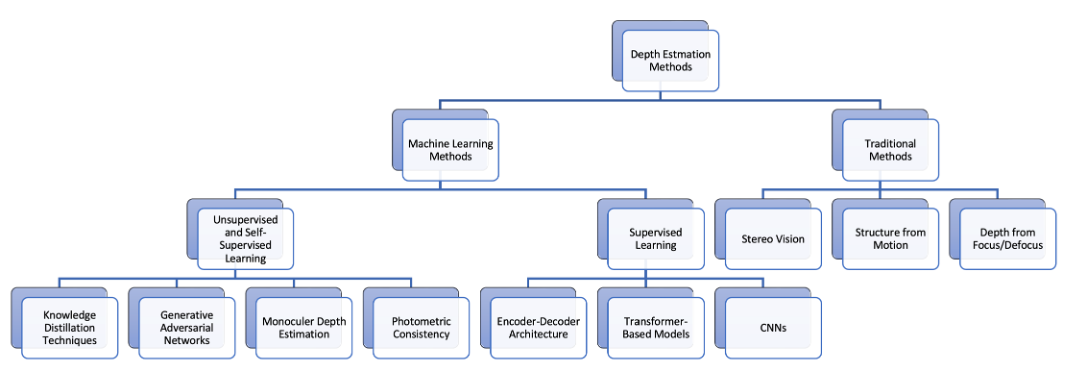
\includegraphics[width=\textwidth]{images/flowchart.png}
    \caption{Methods of Depth Estimation.}
    \label{fig:depth_methods_flowchart}
\end{figure}

\section{Traditional Methods}
\label{sec:traditional_methods}

Traditional methods relied on geometric principles to infer depth. The most important of these are:

\begin{itemize}
    \item \textbf{Stereo Vision:} This technique uses two or more cameras to capture images from slightly different viewpoints and then calculates a depth map through triangulation, as shown in figure \ref{fig:stereo_vision_diagram}. This method requires precise calibration and faces difficulties in textureless regions \cite{scharstein2002taxonomy}.
    
    \begin{figure}[htbp!]
        \centering
        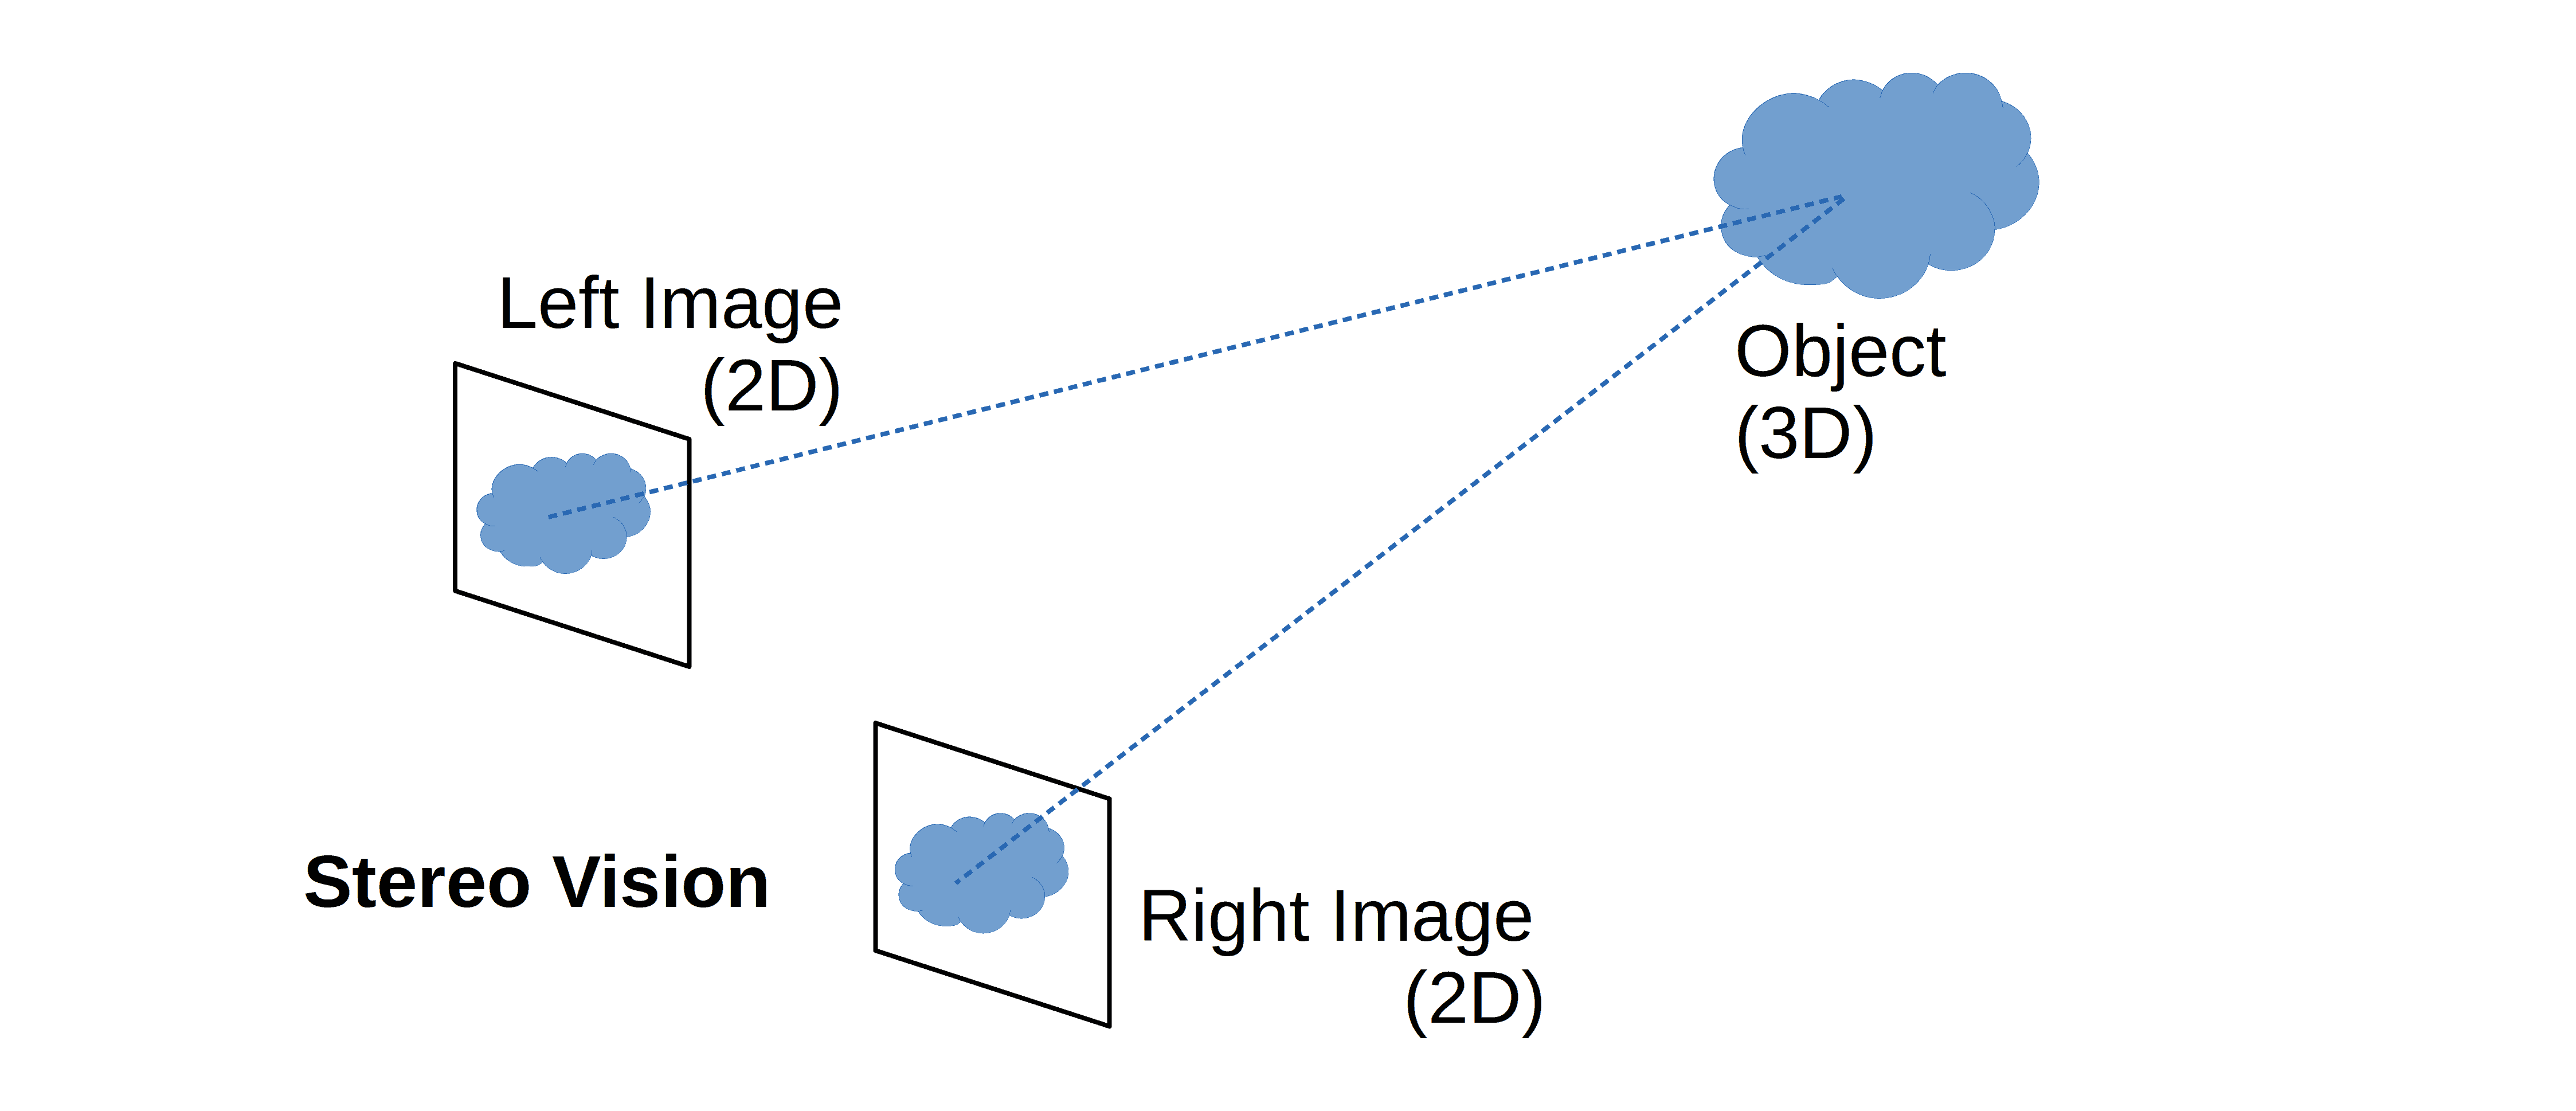
\includegraphics[width=0.8\textwidth]{images/stereo_vision.png}
        \caption{Stereo Vision.}
        \label{fig:stereo_vision_diagram}
    \end{figure}

    \item \textbf{Structure from Motion (SfM):} SfM estimates depth by analyzing the movement of distinctive points across a series of images, which allows for the reconstruction of the scene's 3D structure, demonstrated in figure \ref{fig:sfm_diagram}. This method is sensitive to tracking errors and is computationally expensive \cite{hartley2003multiple,saxena20083}.
    
    \begin{figure}[htbp!]
        \centering
        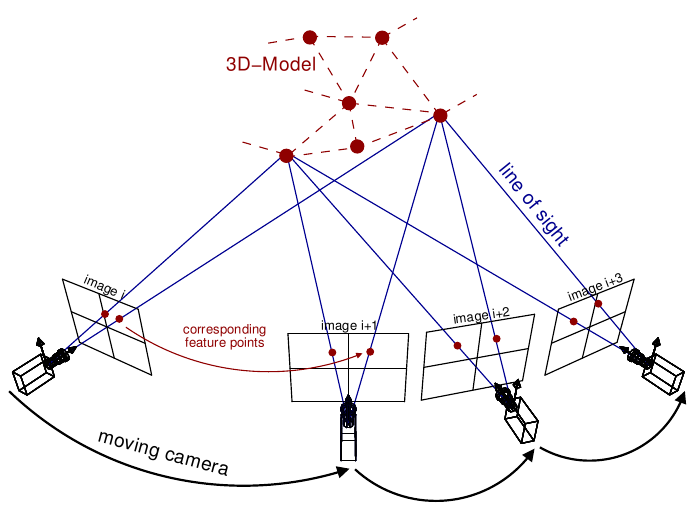
\includegraphics[width=0.9\textwidth]{images/sfm_diagram.png}
        \caption{Structure from Motion.}
        \label{fig:sfm_diagram}
    \end{figure}

    \item \textbf{Depth from Focus/Defocus:} This technique estimates depth based on the degree of blur (defocus) in an image at different focal lengths, as shown in figure \ref{fig:dfd_diagram}. However, this method requires controllable lighting conditions and is limited to the camera's depth of field \cite{pentland1987new}.
    
    \begin{figure}[htbp!]
        \centering
        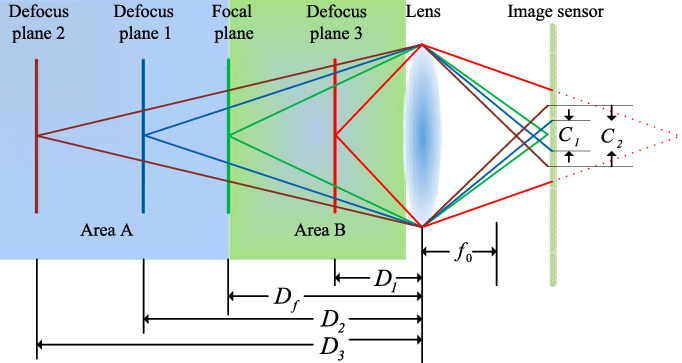
\includegraphics[width=\textwidth]{images/dfd_diagram.png}
        \caption{Depth from Focus/Defocus.}
        \label{fig:dfd_diagram}
    \end{figure}
\end{itemize}

\section{Machine Learning Methods}
\label{sec:deep_learning_methods}

Machine learning models, especially deep learning, have brought about a paradigm shift in the field. They can be divided into:

\subsection{Supervised Learning}
\label{subsec:supervised}

Supervised learning methods require datasets labeled with ground-truth depth maps. These methods have achieved advanced performance by leveraging large-scale datasets and advanced neural network architectures. Key architectures in this approach include:

\begin{itemize}
    \item \textbf{Convolutional Neural Networks (CNNs):} One of the first deep learning models for depth estimation used a multi-scale CNN to predict depth from a single image \cite{eigen2014depth}. This model demonstrated the potential of deep learning for this task.
    \item \textbf{Encoder-Decoder Architectures:} Architectures like U-Net and its variants are widely used for dense depth prediction. These structures combine high-level semantic features with low-level spatial details to produce accurate depth maps \cite{ronneberger2015u}.
    \item \textbf{Transformer Models:} Recent works have discussed the use of Vision Transformers (ViTs) in depth estimation applications \cite{ranftl2021vision}. Transformers capture global context more effectively than CNNs, leading to improved performance in complex scenes.
    \item \textbf{Foundation Models for Depth Estimation:} Early foundational work like MVSNet, an end-to-end deep learning architecture for inferring depth maps from multi-view images \cite{yao2018mvsnet}. More recent work like Depth Anything combines a ViT-L/DPT architecture with DINOv2 pre-training and an affine-invariant loss, achieving state-of-the-art performance without fine-tuning. Its main innovation lies in scaling up to 62 million unlabeled images via automated pseudo-labeling \cite{yang2024depth}.
\end{itemize}

\subsection{Unsupervised and Self-Supervised Learning}
\label{subsec:unsupervised}

Unsupervised and self-supervised methods do not require ground-truth depth maps, making them more scalable and practical for real-world applications. They rely on concepts such as:

\begin{itemize}
    \item \textbf{Photometric Consistency:} This relies on minimizing the photometric error between the original and predicted images using the predicted depth and camera pose. This approach leverages geometric constraints to train the model without labeled data \cite{godard2017unsupervised}.
    \item \textbf{Generative Adversarial Networks (GANs):} GANs have been used to generate realistic depth maps by learning the data distribution \cite{xu2022unsupervised}. These models can improve the quality of depth predictions through adversarial training.
    \item \textbf{Distillation Techniques:} A pre-trained model is used to produce semi-reliable depth maps, and the target model is trained on them \cite{he2025distill}. The student model is typically smaller than the pre-trained teacher model.
\end{itemize}

\begin{table}[htbp!]
    \centering
    \caption{Traditional VS Machine Learning Methods for Depth Estimation.}
    \label{tab:method_comparison}
    \begin{tabularx}{\textwidth}{l >{\RaggedRight}X >{\RaggedRight\arraybackslash}X}
        \toprule
        \textbf{Criterion} & \textbf{Traditional Methods} & \textbf{Machine Learning} \\
        \midrule
        Accuracy & Good & High (with sufficient training) \\
        \addlinespace
        Data Requirement & No need for training data & Requires huge amounts of labeled data for supervised learning and unlabeled data for unsupervised ones \\
        \addlinespace
        Speed & Generally slow but can be real-time & Faster than traditional methods, but requires computational resource \\
        & (e.g., Stereo Vision) & \\
        \bottomrule
    \end{tabularx}
\end{table}

\section{Evaluation Metrics}
\label{sec:evaluation_metrics}
The performance of depth estimation models is evaluated using a variety of metrics, including \cite{gurram2023metrics}:
\begin{itemize}
    \item \textbf{Absolute Relative Difference (Abs Rel):} Measures the relative difference between the predicted and ground-truth depth.
    \item \textbf{Squared Relative Difference (Sq Rel):} Measures the square of the relative difference, emphasizing larger errors.
    \item \textbf{Root Mean Squared Error (RMSE):} Calculates the square root of the average of squared differences.
    \item \textbf{Scale-Invariant Logarithmic Error (SILog):} Accounts for the scale ambiguity in monocular depth estimation, where we know the relative depth between objects but not the absolute metric depth.
    \item \textbf{Accuracy Threshold ($\delta$):} The percentage of pixels where the predicted depth is within a certain threshold of the ground-truth depth, such as $\delta < 1.25$.
\end{itemize}

\section{Datasets for Depth Estimation}
\label{sec:datasets}

The availability of high-quality datasets has been crucial for the advancement of depth estimation. Key datasets include:
\begin{itemize}
    \item \textbf{KITTI:} A widely used dataset for autonomous driving \cite{geiger2012we}, providing stereo images and LiDAR-based depth maps.
    \item \textbf{NYU Depth V2:} An indoor dataset captured with a Microsoft Kinect, containing RGB-D images \cite{silberman2012indoor}.
    \item \textbf{Make3D:} An outdoor dataset containing scenes with laser-scanned depth maps \cite{saxena20083}.
    \item \textbf{Cityscapes:} A large-scale dataset for urban scene understanding, which includes depth maps \cite{cordts2016cityscapes}.
    \item \textbf{COCO:} Although primarily for object recognition, its diversity can be leveraged for depth estimation \cite{lin2014microsoft}.
\end{itemize}

\section{Lightweight Neural Network Architectures}
\label{sec:architectures}

Designing lightweight neural networks is a cornerstone of AI applications on mobile and resource-constrained devices. While this report focuses on MobileNetV3 and MobileViT-XS, the field is rich with innovative architectures seeking to balance accuracy and computational efficiency. Reviewing these architectures provides deeper context and highlights the reasons for choosing MobileViT as the final encoder.

\begin{enumerate}
    \item \textbf{The MobileNet Family:} The MobileNet series is one of the most famous architectures designed for mobile devices Its core idea is to replace costly traditional convolutions with Depthwise Separable Convolutions. This change significantly reduces the number of parameters and computational operations. MobileNetV3 was considered at the beginning of this project, as this version offers further improvements through architectures enhanced by Neural Architecture Search (NAS) and attention mechanisms (Squeeze-and-Excite) \cite{koonce2021mobilenetv3}.
    \item \textbf{The EfficientNet Architecture:} This introduced a new model scaling approach known as Compound Scaling. Instead of arbitrarily scaling one network dimension (like depth or width), EfficientNet uniformly scales all dimensions (depth, width, and image resolution) in a principled manner. This approach allowed it to achieve superior accuracy with significantly fewer parameters compared to its predecessors \cite{koonce2021efficientnet}.
    \item \textbf{The MobileViT Architecture:} Vision Transformers (ViT) have demonstrated superior ability to capture global context thanks to the self-attention mechanism, but they come at a huge computational cost, making them unsuitable for mobile phones. Herein lies the true strength of MobileViT; it is not just a convolutional or transformer architecture, but a hybrid that combines the best of both worlds \cite{mehta2021mobilevit}:
    \begin{itemize}
        \item \textbf{Local Efficiency of CNNs:} MobileViT uses efficient convolutions in its initial layers to extract local features from the image.
        \item \textbf{Global Capability of Transformers:} It then feeds these local features into lightweight transformer layers specifically designed for mobile phones, allowing the model to understand the relationships between different parts of the image and build a holistic understanding of the scene.
    \end{itemize}
\end{enumerate}

The table \ref{tab:arch_comparison} summarizes the key comparison points between these architectures:

\begin{table}[htbp!]
    \centering
    \caption{Comparison of Lightweight Network Architectures.}
    \label{tab:arch_comparison}

    \begin{tabularx}{\textwidth}{
        >{\bfseries}l 
        >{\RaggedRight}X 
        >{\RaggedRight}X 
        >{\RaggedRight\arraybackslash}X 
    }
        \toprule
        Architecture & Core Principle & Computational Efficiency & Observations from Project Experience \\
        \midrule
        MobileNetV3 & 
        Uses Depthwise Separable Convolutions to reduce computations, with enhancements via NAS and Squeeze-and-Excite mechanisms. &
        Very high; designed to significantly reduce parameters and operations, making it suitable for mobile devices. & 
        Used in initial training attempts, but results were poor as the depth maps lost many fine spatial details. \\
        \addlinespace

        EfficientNet & 
        Adopts "Compound Scaling," which systematically and uniformly scales network depth, width, and resolution. & 
        Extremely efficient, achieving high accuracy with far fewer parameters than preceding models. & 
        Tested, but results were not good for depth estimation. The likely reason is that the architecture focuses on classification and does not preserve the spatial details needed for depth reconstruction. \\
        \addlinespace

        MobileViT & 
        A hybrid architecture combining efficient CNN convolutions for local features and lightweight Transformer layers for global context. &
        Specifically designed to be light, fast, and suitable for mobile phones, while retaining the ability to understand global context via self-attention. & 
        Achieved the best results and was adopted as the final encoder. Its ability to effectively understand global context was what previous attempts lacked. \\
        \bottomrule
    \end{tabularx}
\end{table}
% --- CHAPTER 3 ---
\chapter{Methodology}
\label{chap:methodology}

\section{Technologies Used}
\label{sec:technologies_used}

\begin{enumerate}
    \item \textbf{Knowledge Distillation:} This is the core strategic technique upon which this project is built. It aims to resolve the conflict between the high accuracy of large models and the computational requirements of resource-constrained devices like mobile phones. The fundamental idea is to train a small, efficient model (the "student model") to mimic the behavior and outputs of a large, high-performance model (the "teacher model") \cite{hu2023teacher}.
    \item \textbf{Model Architecture (Encoder-Decoder):} The model is built upon an encoder-decoder architecture, which is a common design for neural networks used for tasks such as depth estimation. The encoder processes the image to extract features, and the decoder then uses these features to generate the depth map.
    \item \textbf{Vision Transformer (ViT):} This is a neural network architecture that is particularly effective at capturing the global context of an image. The teacher model, \textbf{Depth Anything V2}, is based on this technology.
\end{enumerate}

\section{Knowledge Distillation Technique}
\label{sec:kd_technique}

Knowledge Distillation is a form of \textbf{Model Compression} in Machine Learning \cite{hinton2015distilling}. It aims to transfer "knowledge" from a large, complex, high-performance "teacher" model to a smaller, more computationally efficient "student" model. The idea is inspired by the real-world teacher-student relationship, where a teacher not only gives the student the final answer but also explains the thinking and logic that lead to it. The primary objective is to create a compact model with a small memory footprint and fast inference speed, making it suitable for deployment on mobile devices.

\subsection{Distillation Mechanism}
\label{subsec:distillation_mechanism}

The distillation mechanism relies on training the student model not only on the original labeled data ("hard targets") but also on the outputs of the teacher model. The power of this technique lies in the fact that the teacher model provides richer training signals than just the correct answer alone \cite{hu2023teacher}.

\begin{enumerate}
    \item \textbf{Hard Targets:} These are the correct, ground-truth labels from the dataset (e.g., this image contains a cat). Training a small student model exclusively on hard targets can be challenging, as the model may lack the capacity to learn the complex underlying function perfectly.
    \item \textbf{Soft Targets:} These are the complete probabilistic outputs of the teacher model. For example, in a simple classification problem, instead of saying "this is a cat," the teacher might say, "this is 90\% a cat, 6\% a dog, 4\% a rabbit, etc." This probability distribution, known as \textbf{"dark knowledge,"} contains rich, implicit information about the similarity between different classes from the teacher's perspective. When the student learns to mimic these "soft targets," it learns the relational structure between classes, leading to better generalization and higher performance.
\end{enumerate}

\subsection{Types of Distillable Knowledge}
\label{subsec:types_of_knowledge}

The process of distillation is not limited to the final output layer. Multiple types of knowledge can be transferred to enhance the student's performance \cite{hu2023teacher}:
\begin{itemize}
    \item \textbf{Response-Based Distillation:} This is the classic form of distillation, where the student model is trained to directly mimic the final prediction ("soft targets") of the teacher model.
    \item \textbf{Feature-Based Distillation:} In this type, the student model is trained to replicate the intermediate feature maps produced by the teacher's hidden layers. This forces the student to learn the same feature-extraction hierarchy that the teacher uses, helping it to understand the data more deeply.
    \item \textbf{Relation-Based Distillation:} This approach focuses on distilling the relationships between data points or feature maps, such as by having the student model mimic the teacher's attention maps or the correlation matrices between features.
\end{itemize}

\section{Training Methodology}
\label{sec:training_methodology}

The training approach is based on a teacher-student framework to distill and compress the knowledge from the large model to the smaller one.

\begin{itemize}
    \item \textbf{Teacher Model:} The \textbf{Depth Anything V2 (Small)} model is used as the teacher. This model is pre-trained on a massive dataset and produces high-quality depth estimation results, but its large size and computational requirements make it unsuitable for mobile devices.
    \item \textbf{Student Model:} A new, lightweight student model was designed with an architecture such as \textbf{MobileViT-XS}. Its architecture was chosen to have a low parameter count, enabling fast and efficient inference.
\end{itemize}

The distillation process is guided by training the student model to minimize a composite \textbf{Loss Function}. In our case, the loss function consists of four components:

\begin{enumerate}
    \item \textbf{Scale-Invariant Logarithmic Loss (SILog):} This is the primary component, which measures the accuracy of the student's predicted depth map ($d$) compared to the teacher's output ($d^*$). This loss uses a scale-invariant logarithmic scale to ensure structural correctness \cite{eigen2014depth}.
    
    The loss is calculated using the following formula:
    \begin{equation}
        L_{\text{silog}} = \frac{1}{N}\sum_{i} (\log(d_i) - \log(d_i^*))^2 - \frac{1}{N^2} (\sum_{i} (\log(d_i) - \log(d^*_i)))^2
        \label{eq:silog}
    \end{equation}
    
    where $d_i$ and $d_i^*$ are the predicted and teacher depths for each pixel $i$, and $N$ is the total number of pixels. This loss ensures that the structure of the predicted depth map is correct, regardless of the overall scale.  Demonstrated in Figure~\ref{fig:silog_diagram}

    \begin{figure}[htbp]
        \centering
        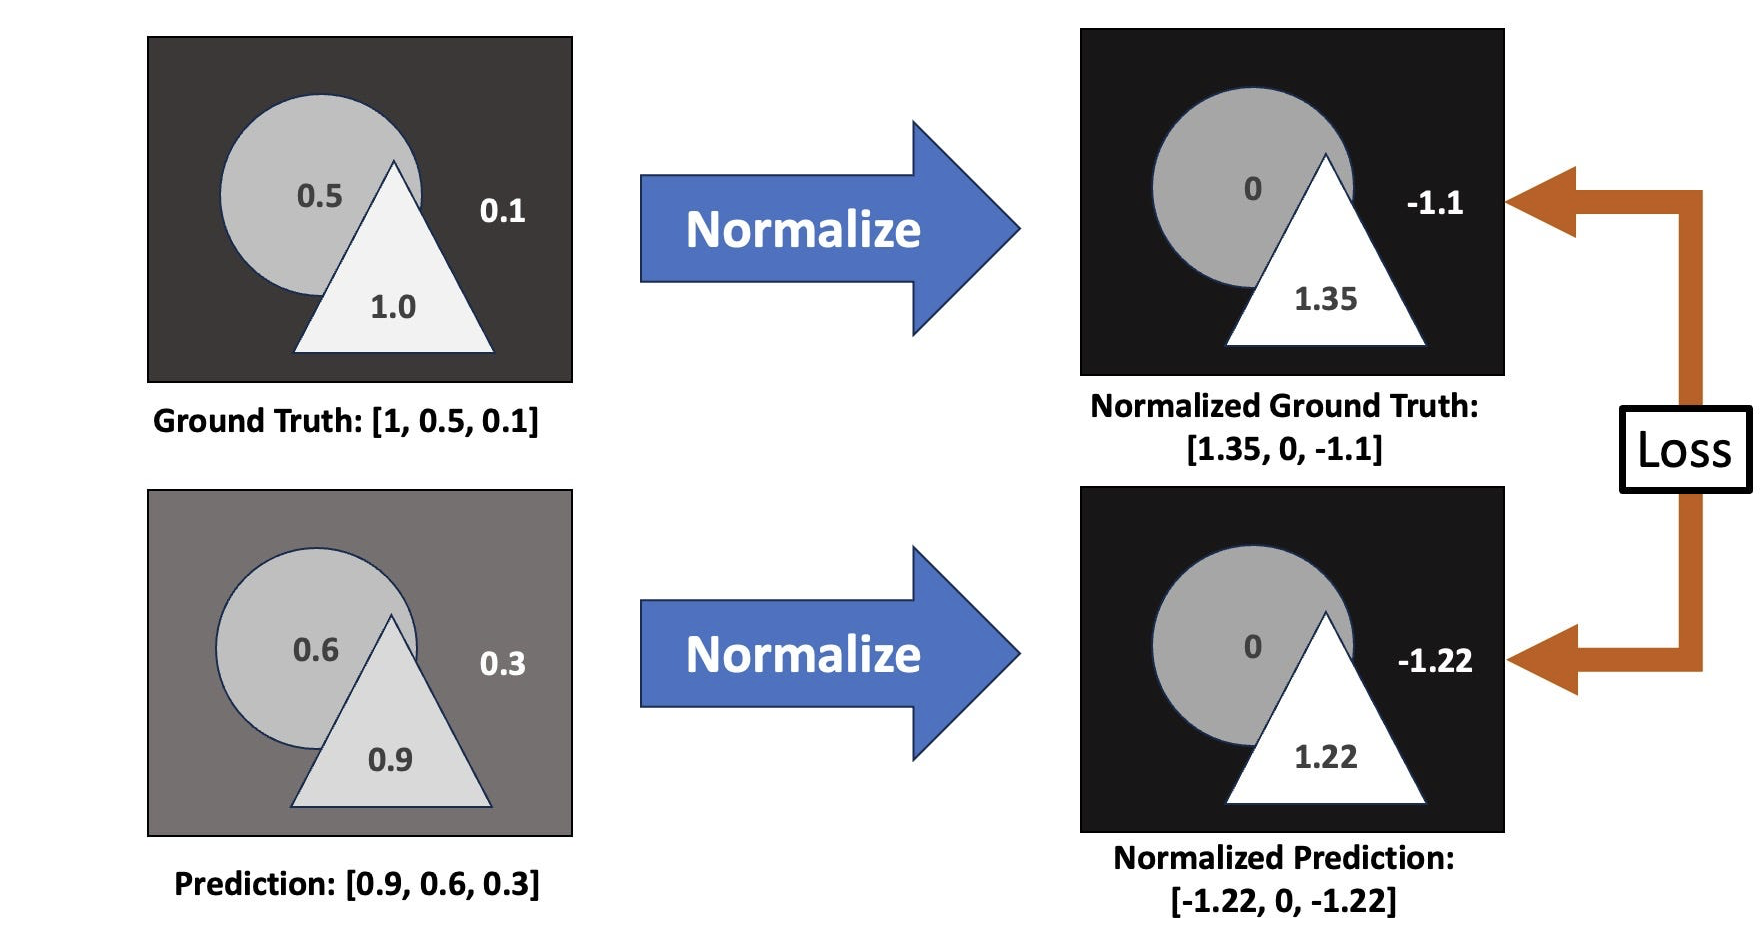
\includegraphics[width=0.8\textwidth]{images/silog_diagram.png}
        \caption{Scale-Invariant Logarithmic Loss.}
        \label{fig:silog_diagram}
    \end{figure}

    \item \textbf{Gradient Matching Loss:} This loss component forces the gradients of the student's depth map to be similar to the gradients of the teacher's depth map. This is crucial for preserving the edges and fine-grained details of the scene \cite{li2018megadepth}.
    
    The loss is calculated as the L1 distance between the teacher and student gradients:
    \begin{equation}
        L_{\text{grad}} = \frac{1}{N} \sum_i \left( |\nabla_x(d_i) - \nabla_x(d_i^*)| + |\nabla_y(d_i) - \nabla_y(d_i^*)| \right)
        \label{eq:grad_loss}
    \end{equation}
    where $d_i$ is the student's prediction, $d_i^*$ is the teacher's prediction, $\nabla_x$ and $\nabla_y$ are the gradient operators (e.g., Sobel filters) in the horizontal and vertical directions  (demonstrated in Figure~\ref{fig:gradient_loss_diagram}), and $N$ is the total number of pixels.

    \begin{figure}[htbp]
        \centering
        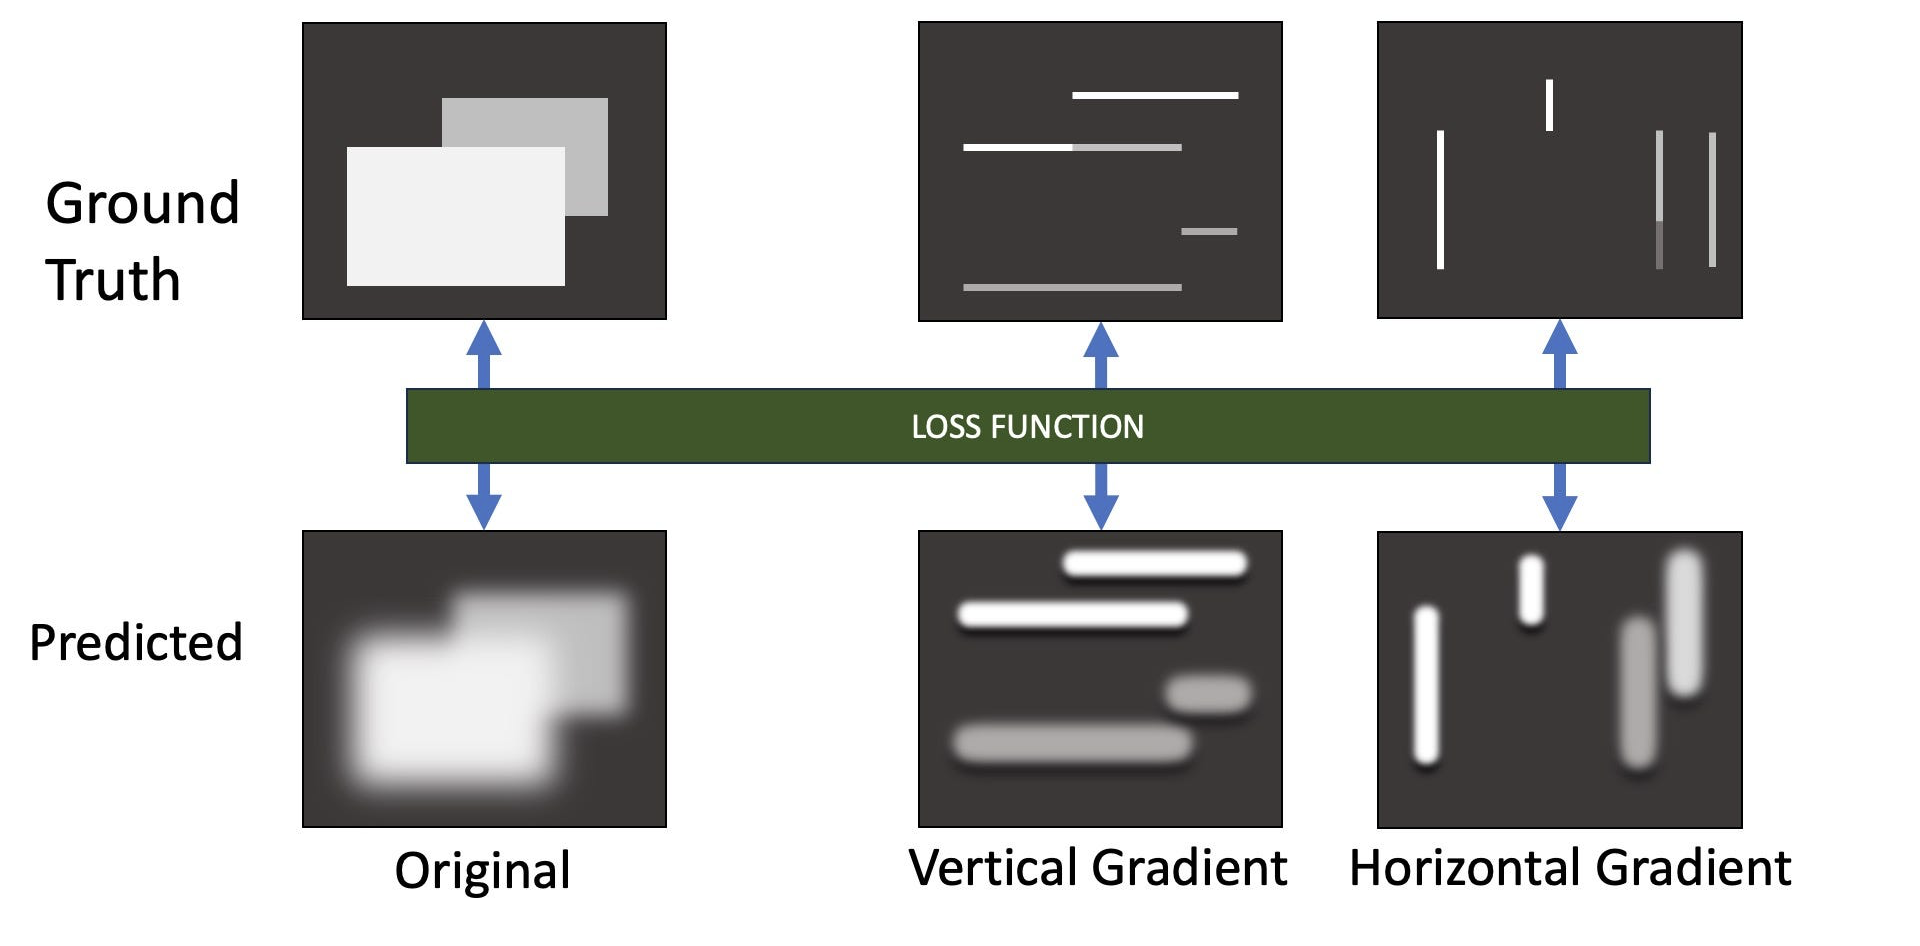
\includegraphics[width=\textwidth]{images/gradient_loss_diagram.png}
        \caption{Gradient Matching Loss.}
        \label{fig:gradient_loss_diagram}
    \end{figure}

    \item \textbf{Feature Matching Loss:} Instead of only mimicking the final output, this loss aims to make the student's intermediate feature maps ($f_i^S$) similar to the teacher's ($f_i^T$). This helps the student learn the "internal representations" that the teacher uses to understand the scene~\cite{hu2023teacher}.
    \begin{equation}
        L_{\text{feat}} = \frac{1}{M} \sum_{i} |f_i^S - f_i^T|
        \label{eq:feat_loss}
    \end{equation}
    where $M$ is the number of features in the feature maps.

    \item \textbf{Attention Matching Loss:} This loss computes a simplified "attention map" for both the student ($attn^S$) and the teacher ($attn^T$) by summarizing their feature maps. By matching these maps, the student is encouraged to focus on the same important spatial regions in the image as the teacher~\cite{hu2023teacher}.
    
    The attention map is generated efficiently and directly by summarizing information across the channel dimension of a feature map. The process is as follows:
    \begin{enumerate}
        \item \textbf{Calculate Absolute Value:} First, the absolute value of all values in the feature map is taken. This ensures that strong activations, whether positive or negative, contribute positively to identifying regions of interest.
        \item \textbf{Average Across Channels:} Next, the average of the values is computed across the channel dimension for each spatial location. This "compresses" the multiple feature maps into a single 2D map representing the relative spatial importance of each region.
    \end{enumerate}
    
    Mathematically, the value of a pixel in the final attention map $attn$ at spatial location $(i,j)$ can be expressed as follows, where $f_{c,i,j}$ is the pixel value in channel $c$ at location $(i,j)$ and $C$ is the total number of channels:
    \begin{equation}
        attn_{i,j} = \frac{1}{C}\sum_{c=1}^{C}|f_{c,i,j}|
    \end{equation}
    
    The loss is then calculated as:
    \begin{equation}
        L_{\text{attn}} = \frac{1}{M'}\sum_{i}(attn^S - attn^T)^2
        \label{eq:attn_loss}
    \end{equation}
\end{enumerate}

These losses are combined into a single total loss function using weighting coefficients ($\lambda$) for each component:
\begin{equation}
    L_{\text{total}} = \lambda_{\text{silog}}L_{\text{silog}} + \lambda_{\text{grad}}L_{\text{grad}} + \lambda_{\text{feat}}L_{\text{feat}} + \lambda_{\text{attn}}L_{\text{attn}}
    \label{eq:total_loss}
\end{equation}
The weighting coefficients will be tuned during practical implementation based on experimental results.

\section{The Student Model (Delta) Design}
\label{sec:delta_model_design}

Several models were designed and tested by changing the encoder or the decoder structure, but we will only describe the final adopted model. The design and development of the student model, named \textbf{Delta ($\Delta$)}, was an iterative process of experimentation and refinement to achieve the best balance between performance and efficiency.

\subsection{Teacher Model Architecture}
\label{subsec:teacher_arch}

The teacher model is \textbf{Depth Anything V2}, which is based on a \textbf{Vision Transformer (ViT)} architecture, specifically \textbf{DINOv2}, The Figure~\ref{fig:teacher_arch} shows the Depth Anything architecture. This model excels at extracting rich and contextual features from the entire image, giving it superior accuracy in depth estimation. It consists of a large ViT-based encoder and a subsequent set of decoder layers that transform these features into a depth map~\cite{yang2024depth,yang2024depthV2}. Its large size makes it impractical for mobile applications. It is worth noting that any inaccuracies in the teacher model's predictions can be propagated to the student during training.

\begin{figure}[htbp!]
    \centering
    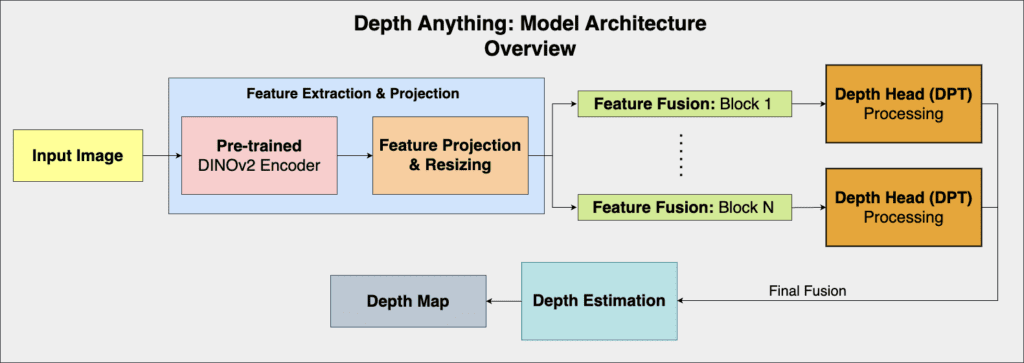
\includegraphics[width=\textwidth]{images/teacher_model_arch.png}
    \caption{Teacher Model Architecture.}
    \label{fig:teacher_arch}
\end{figure}

\subsection{Student Model (Delta) Architecture}
\label{subsec:student_arch}

The student model was designed to achieve a balance between accuracy and inference speed on mobile devices. Taking into consideration that for knowledge distillation, it is often beneficial to design a student architecture that mimics the teacher's structure, the student consists of two main parts (As shown in Figure \ref{fig:delta_arch}):

\begin{enumerate}
    \item \textbf{The Encoder:} The \textbf{MobileViT-XS} architecture was chosen as the encoder for the student model. MobileViT is a hybrid model that combines the efficiency of Convolutional Neural Networks (CNNs) in extracting local features with the ability of Vision Transformers to understand the global context of the image. This architecture makes it lightweight, fast, and ideal for running on mobile phones. The version pre-trained on the ImageNet dataset was used to extract basic features~\cite{mehta2021mobilevit}.

    \item \textbf{The Decoder:} A custom, lightweight decoder module, named \textbf{MiniDPT}, was designed. It is inspired by the DPT architecture~\cite{ranftl2021vision} but with significant simplifications to reduce computational complexity. The decoder receives multi-scale feature maps from the encoder and progressively fuses them to produce the final depth map. This process occurs in three stages:

    \begin{description}
        \item[Projection Stage:] Before fusion begins, each feature map coming from the encoder is processed separately. A \texttt{1x1 convolution}, followed by \texttt{Batch Norm} and a \texttt{ReLU} activation, is applied to each feature map. The goal of this stage is to unify the number of channels across the encoder's feature maps to match the required dimensions for each stage of the decoder.

        \item[Upsampling \& Fusion Stage:] This is the core stage of the decoder. It is an iterative process, starting from the feature map with the lowest spatial resolution (most abstract) and progressing to the highest resolution. In each step of the iteration, two main blocks are applied:
        \begin{enumerate}
            \item \textbf{Upsample Block:} This block is responsible for increasing the spatial resolution. It uses an \texttt{nn.Upsample} layer with bilinear interpolation to double the map's dimensions. Then, for high computational efficiency, the upsampled features are processed using \textbf{Depthwise Separable Convolutions} instead of traditional convolutions. This design choice is crucial for reducing the number of parameters and making the model lightweight.
            \item \textbf{Fusion Block:} This block implements a skip-connection mechanism. It fuses the output from the Upsample Block with the corresponding feature map coming from the "Projection Stage". The fusion is performed via concatenation (\texttt{torch.cat}) along the channel dimension, followed by a series of convolutional layers (\texttt{1x1 Conv}, \texttt{Batch Norm}, \texttt{ReLU}) to process and refine the combined features.
        \end{enumerate}
        This gradual fusion allows the model to combine high-level semantic information from deep layers with fine spatial details from shallow layers.

        \item[Prediction Head:] After the final fusion stage, the resulting feature map is processed through a series of layers to generate the final output. The prediction head consists of \texttt{Conv2d} layers, \texttt{ReLU}, and a final \texttt{Upsample} layer, ending with a \texttt{Conv2d} layer with a kernel size of 1 to produce a single-channel map. A \texttt{Sigmoid} activation function is then applied to ensure the output depth values are normalized between 0 and 1.
    \end{description}
\end{enumerate}

The final student model consists of \textbf{3,373,265} parameters (~3.4 million). In comparison, the teacher model has \textbf{24.8 million} parameters, making our student model approximately \textbf{1/7th} the size of the teacher model.


\begin{figure}[htbp!]
    \centering
    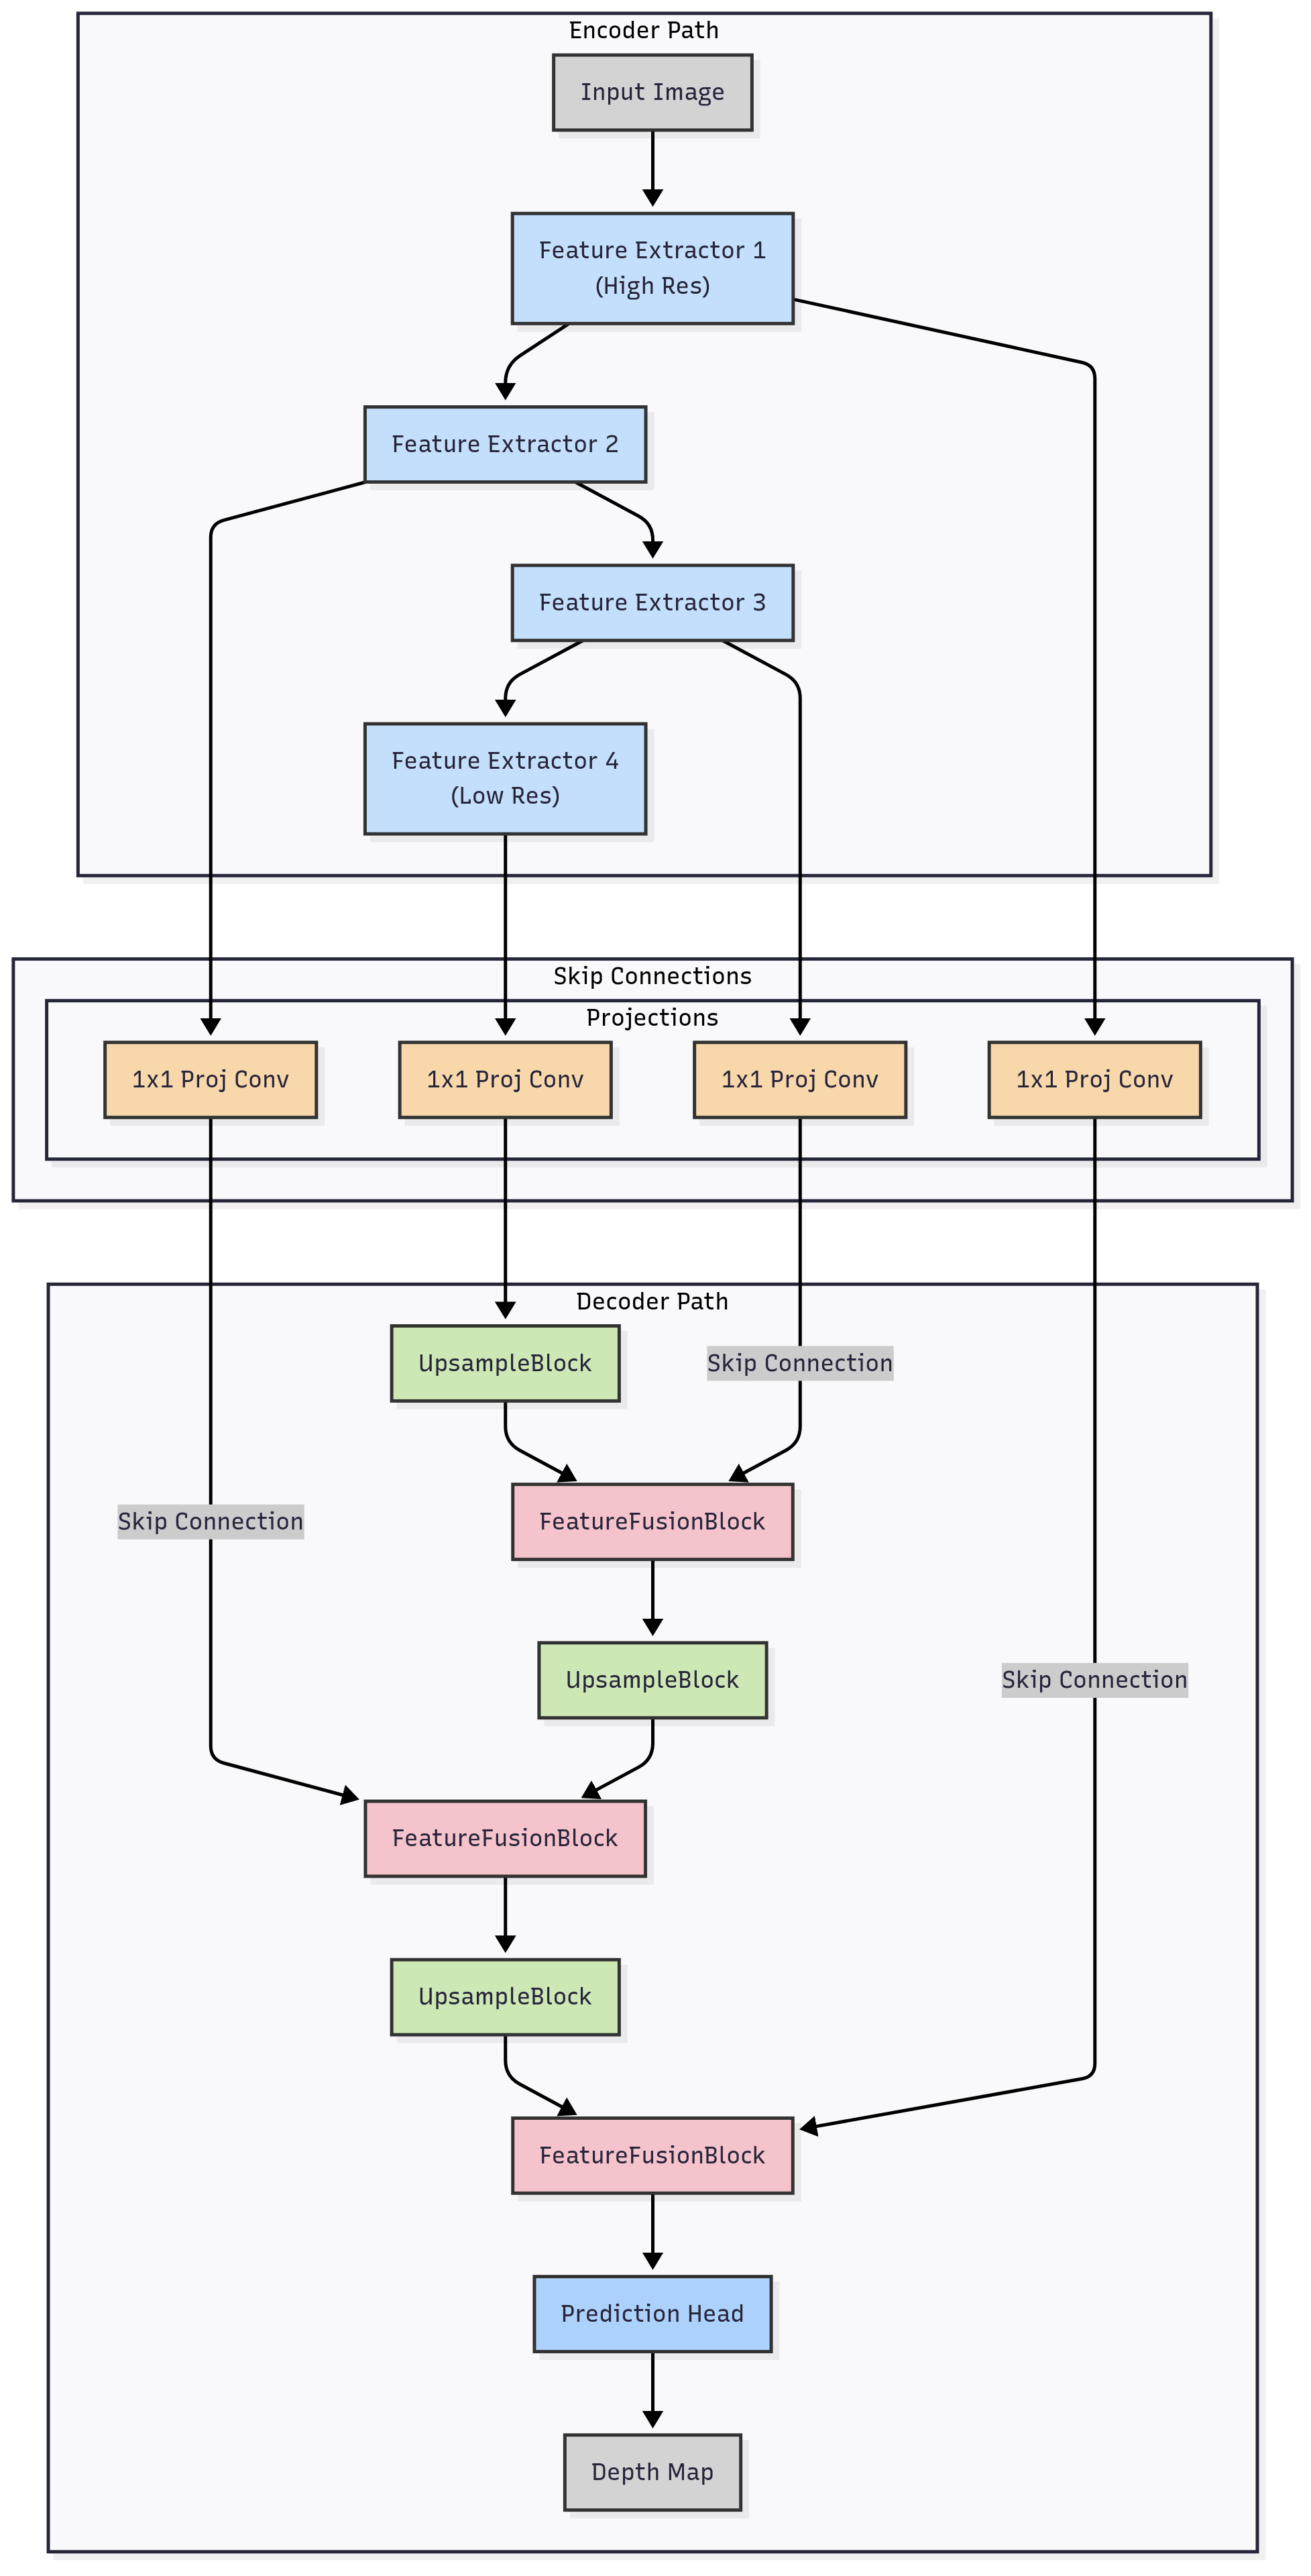
\includegraphics[width=0.9\textwidth, height=0.9\textheight]{images/delta_arch.png}
    \caption{Student Model (Delta) Architecture}
    \label{fig:delta_arch}
\end{figure}
% --- CHAPTER 4 ---
\chapter{Implementation and Application}
\label{chap:implementation}

\section{Environments and Tools Used}
\label{sec:tools}

The development and training of the student model, in addition to the creation of the mobile application, relied on a set of modern and effective tools and technologies:

\begin{enumerate}
    \item \textbf{PyTorch Framework:} Chosen for its flexibility and ease of use in building and training deep learning models, in addition to its extensive support from the scientific community and available resources.
    \item \textbf{Flutter Development Kit:} Used to build the cross-platform mobile application for both Android and iOS from a single codebase, which simplifies the development and deployment process. It was specifically chosen for its libraries that support running AI models in the ONNX format.
    \item \textbf{VS Code Editor:} An advanced code editor used for writing all the project's source code. Its support for a wide range of languages and features through diverse extensions makes it highly effective.
    \item \textbf{GIT Version Control:} A version control system used to track changes to the software during development. This tool facilitates error detection and rollbacks, allowing us to maintain multiple versions of the program and revert to any of them if needed.
    \item \textbf{ONNX (Open Neural Network Exchange):} An open file format used to run trained artificial intelligence models. Flutter contains libraries that support running models in this format, which was crucial for deploying the model on a mobile device.
    \item \textbf{Teacher Model (Depth Anything V2 Small):} This is the specific, pre-trained "teacher" model used to provide the expertise that is "distilled" to the student model.
    \item \textbf{MobileNetV3 Architecture:} An efficient Convolutional Neural Network (CNN) architecture designed specifically for mobile and resource-constrained devices. It was considered as an encoder for the student model due to its lightweight structure and its ability to achieve a good balance between accuracy and inference speed~\cite{koonce2021mobilenetv3}. This was one of the attempts before adopting the final MobileViT-XS architecture.
    \item \textbf{MobileViT-XS Architecture:} The specific neural network architecture chosen as the encoder for the lightweight student model. It is a hybrid architecture that combines the efficiency of CNNs with the power of Vision Transformers~\cite{mehta2021mobilevit}, making it ideal for mobile devices.
    \item \textbf{Google Colaboratory (Colab):} A cloud-based development environment based on Jupyter notebooks. It was used in this project to train the deep learning model. The platform provided access to high-performance computing resources, specifically Graphics Processing Units (GPUs), which significantly accelerated the model training process and allowed for efficient experimentation with different architectures and configurations without the need for expensive local hardware.
\end{enumerate}

\section{Model Building and Training}
\label{sec:model_building}

\subsection{Environment Setup}
\label{subsec:env_setup}

A dedicated virtual environment was created for the project. This environment contains a specific Python interpreter along with libraries and files isolated from other projects, preventing conflicts between package versions. After activating the environment, all required libraries defined in the \texttt{requirements.txt} file were installed to execute the code for building and training the model.

\subsection{File Structure}
\label{subsec:file_structure}

The project was organized with the following clean file structure:
\begin{description}
    \item[\texttt{Config}:] This folder contains all constants and general information utilized across the project, such as model paths, appropriate image dimensions, transformations applied to images before training and testing, and the selected weighting coefficients for the loss function.
    \item[\texttt{notebooks}:] Contains Jupyter notebooks that were executed on Google Colab for training and testing specific model architectures or loss functions, due to the lack of available local hardware resources.
    \item[\texttt{Models}:] This folder contains the source code for the student and teacher model architectures. Notably, the \textit{Factory} design pattern was used to allow for easily swapping different architectures for the student or teacher. This ensures a clean codebase where only a few lines need to be changed in \texttt{factory.py} and \texttt{config.py}, leaving the files that use the models unchanged.
    \begin{itemize}
        \item \textbf{For the Teacher:} A \texttt{class} was built to wrap the pre-trained model to normalize its output and extract internal feature maps. An image is passed to the pre-trained model, and feature maps from specific layers are extracted to serve as learning targets for the student. These features are then reshaped to a format the student understands (bridging the technical gap between how Transformers and CNNs process information). Finally, the output depth map is normalized so its pixel values are between 0 and 1.
        \item \textbf{For the Student:} Several architectures were tested. The final version is distributed across four classes:
        \begin{itemize}
            \item \texttt{UpsampleBlock}: Defines the upsampling block used in the decoder. It doubles the spatial resolution of the input and uses \textit{Depthwise Separable Convolutions}, which are highly efficient as they significantly reduce the number of computational operations and model size compared to traditional convolutions.
            \item \texttt{FeatureFusionBlock}: Defines the feature fusion block in the decoder. It merges high-level features from the decoder stage with low-level features from the encoder stage, effectively acting as our implementation of skip-connections.
            \item \texttt{MiniDPT}: Represents the decoder. It mimics the decoder used in the teacher model but is much lighter. It projects the feature maps from the encoder to match the decoder's dimensions and is defined recursively with several layers of the two blocks described above. Finally, a prediction head with a \texttt{Sigmoid} activation function is used to output the final depth map with values between 0 and 1.
            \item \texttt{StudentDepthModel}: This class uses the pre-trained encoder (the final design uses MobileViT-XS), extracts internal feature maps from it, passes them to the MiniDPT decoder, and then outputs the final result.
        \end{itemize}
    \end{itemize}
    \item[\texttt{datasets}:] Contains a class for loading the training and testing datasets and applying the desired transformations (\texttt{Transforms}).
    \item[\texttt{data}:] Contains a script to rename images with a numbered naming convention and an \texttt{images} subfolder holding all the images the model was trained on, which were collected with the help of friends.
    \item[\texttt{criterion}:] Here, the loss functions are defined. Due to the need to test several loss functions, the \textit{Factory} and \textit{Strategy} design patterns were used to allow for changing the loss function with great flexibility by modifying a single line in \texttt{config.py}. The primary function used is defined in the \texttt{CombinedDistillationLoss} class, which implements what was theoretically defined in Section~\ref{sec:training_methodology}.
    \item[\texttt{utils}:] Contains helper tools for training and use. It also uses a \textit{Factory} pattern to allow for selecting different optimizers and defines the transformations applied to images before they are fed into the model. It also contains \texttt{metrics.py} for calculating the evaluation metrics for the depth map based on the criteria mentioned in the theoretical study.
    \item[\texttt{scripts}:] This folder contains scripts that perform a complete pipeline:
    \begin{itemize}
        \item A \textbf{training script} that loads the models and dataset, performs the training, and saves the best model based on the loss value on a dedicated validation set.
        \item An \textbf{evaluation script} that shows the model's performance according to the metrics defined in the theoretical study(See Section~\ref{sec:evaluation_metrics}).
        \item An \textbf{inference script} that uses the specified model to generate depth maps for one or more specified images.
        \item A \textbf{conversion script} to convert the model from \texttt{.pth} format to \texttt{.onnx}, which is useful at the deployment stage.
    \end{itemize}
    \item[\texttt{tests}:] This folder contains tests. Unit testing was defined for every module in the program under various edge cases. Afterward, integration testing was performed between these modules by testing a complete, miniature training pipeline.
\end{description}

\subsection{Training Attempts}
\label{subsec:training_attempts}

Several experiments were conducted to improve the model's performance and design. In this phase, training was conducted on a smaller dataset to find the most suitable model before training on a more diverse dataset. The most prominent attempts are summarized below:

\begin{enumerate}
    \item \textbf{Attempt 1: Using MobileNetV3 Encoder}
    The first attempt involved using a \textbf{MobileNetV3-Large} encoder with a simple decoder composed of upsampling and standard convolutional layers. Equal weighting coefficients were used for the components of the loss function.
    \begin{itemize}
        \item \textbf{Observation:} The performance was poor. The resulting depth map, shown in Figure~\ref{fig:attempt1}, lost many details due to the absence of low-level features during the reconstruction process, as shown in Figure~\ref{fig:attempt1}. After this attempt, the loss weights were adjusted to increase the weight of the gradient loss to encourage the model to capture edges, and the SILog loss weight was also increased.
    \end{itemize}

    \begin{figure}[htbp!]
        \centering
        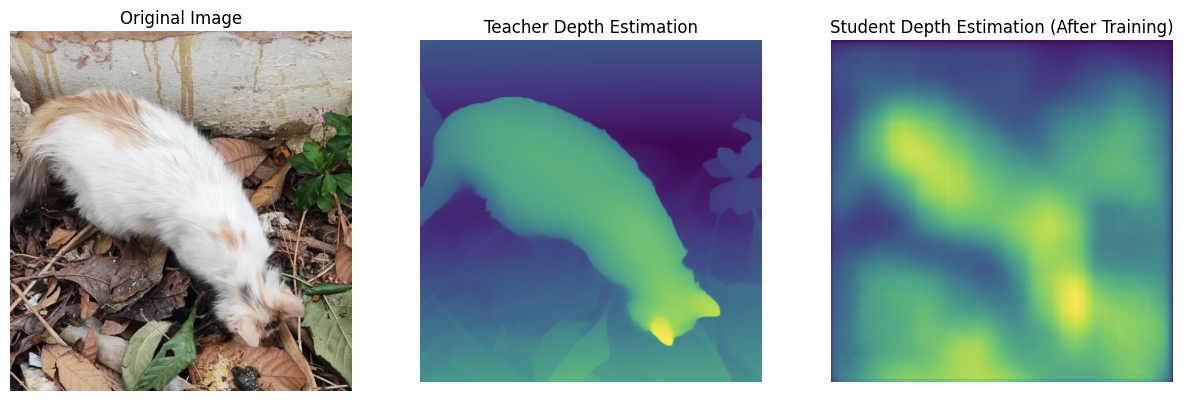
\includegraphics[width=\textwidth]{images/training_attempt_1.png}
        \caption{Results of the First Training Attempt.}
        \label{fig:attempt1}
    \end{figure}
    
    \item \textbf{Attempt 2: Same Encoder with Skip-Connections}
    \begin{itemize}
        \item \textbf{The Architecture:} The same MobileNetV3 architecture was used, but with the addition of skip-connections from different layers in the encoder to the corresponding layers in the decoder.
        \item \textbf{Observation:} A noticeable improvement in the quality of the depth maps was observed (Figure~\ref{fig:attempt2}), as the skip-connections helped in restoring fine spatial details. However, the architecture was still not ideal. The results commonly lacked a sense of \textit{global context}. From this point, we shifted towards using MobileViT as the encoder.
    \end{itemize}

    \begin{figure}[htbp!]
        \centering
        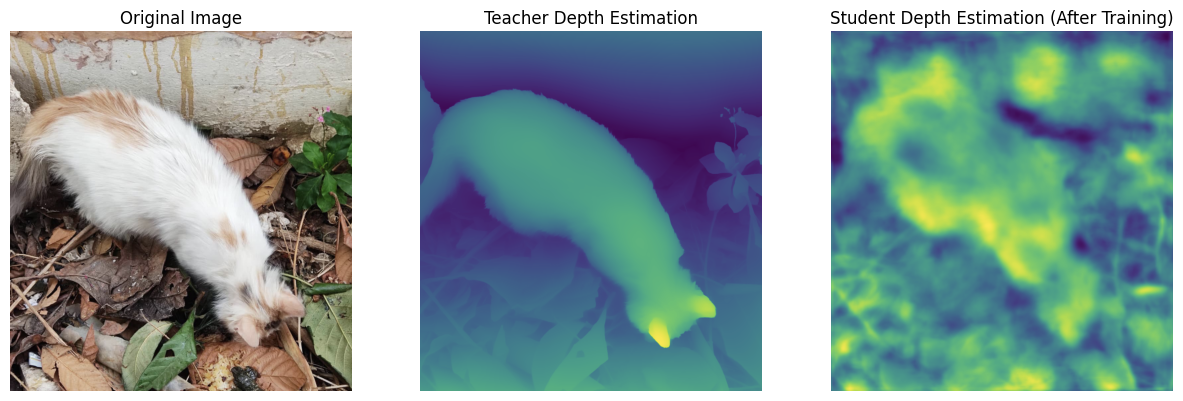
\includegraphics[width=\textwidth]{images/training_attempt_2.png}
        \caption{Results of the Second Training Attempt.}
        \label{fig:attempt2}
    \end{figure}

    \item \textbf{Attempt 3 (Final Model): Using MobileViT}
    This attempt represents the final and best-performing architecture that was adopted.
    \begin{itemize}
        \item \textbf{The Architecture:} The encoder was replaced with \textbf{MobileViT-XS}, and the decoder was the custom \textbf{MiniDPT} described in the file structure section.
        \item \textbf{Training Details:}
        \begin{itemize}
            \item \textbf{Dataset:} Unlabeled images taken with a mobile phone camera.
            \item \textbf{Data Augmentation:} To increase data diversity and prevent overfitting, operations such as horizontal flipping, random rotation, cropping, resizing, and color jittering were applied.
            \item \textbf{Optimizer:} The \textbf{AdamW} optimizer was used with a \textbf{CosineAnnealingLR} learning rate scheduler to dynamically adjust the learning rate during training, which helps in reaching a better convergence point.
            \item \textbf{Loss Function:} The composite loss function was used with the weights shown in Table~\ref{tab:loss_weights}.
        \end{itemize}
    \end{itemize}

    \begin{table}[htbp!]
        \centering
        \caption{Weighting Coefficients for the Composite Loss Function.}
        \label{tab:loss_weights}
        \begin{tabular}{lcccc}
            \toprule
            \textbf{Weight} & $\lambda_{\text{silog}}$ & $\lambda_{\text{grad}}$ & $\lambda_{\text{feat}}$ & $\lambda_{\text{attn}}$ \\
            \midrule
            \textbf{Value}  & 1.5 & 1.5 & 0.5 & 0.4 \\
            \bottomrule
        \end{tabular}
    \end{table}

    \begin{itemize}
        \item[]
        \begin{itemize}
            \item \textbf{Epochs:} The model was trained for \textbf{60 epochs}. An initial learning rate of \textbf{$10^{-3}$} was used for the decoder and \textbf{$10^{-5}$} for the pre-trained encoder.
            \item \textbf{Batch Size:} A batch size of \textbf{12} was used with an image resolution of \textbf{384 x 384} pixels.
            \item \textbf{Observation:} We witnessed a significant improvement in the results, with a better understanding of the global context and an ability to capture edges. However, the model is susceptible to color-based artifacts, occasionally misinterpreting color variations as changes in depth, as seen with the liquid on the wall in Figure~\ref{fig:attempt3}. This limitation likely stems from a lack of diversity or inherent biases in the training data.
        \end{itemize}
    \end{itemize}

    \begin{figure}[htbp!]
        \centering
        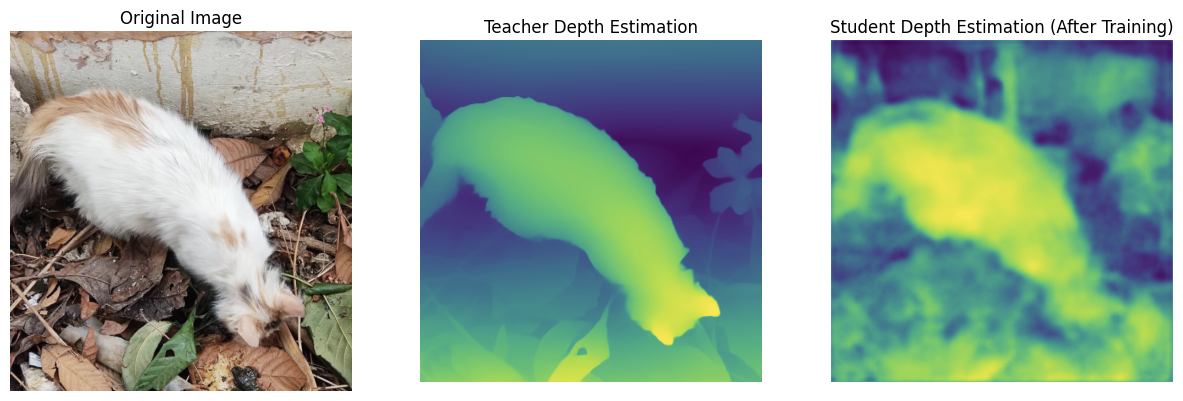
\includegraphics[width=\textwidth]{images/training_attempt_3.png}
        \caption{Results of the Third Training Attempt.}
        \label{fig:attempt3}
    \end{figure}
    
    This model was adopted, and the final training process was conducted on a larger dataset.
\end{enumerate}

\subsection{Tuning the Loss Function Weights}
\label{subsec:loss_tuning}

Initially, equal weights were used for the loss components, but this led to blurry results around the edges, as shown in Figure~\ref{fig:loss_tuning}.

\begin{figure}[htbp!]
    \centering
    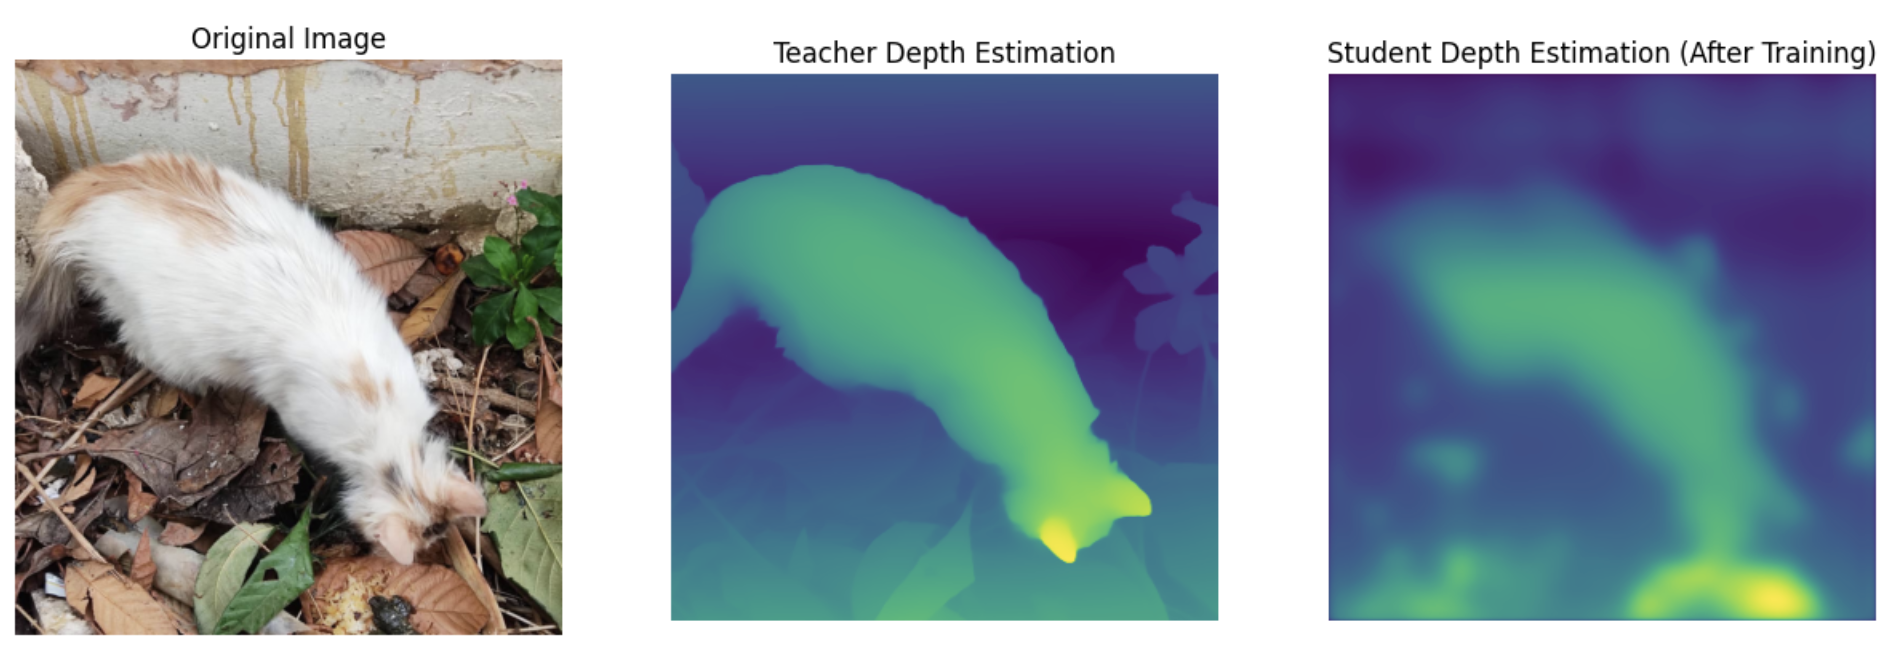
\includegraphics[width=\textwidth]{images/loss_tuning_result.png}
    \caption{Comparison of outputs when using equal weights for loss functions.}
    \label{fig:loss_tuning}
\end{figure}

Based on this, the weight of the gradient loss was gradually increased from 1.0 to 1.5, which showed a marked improvement in preserving details in the validation images. From the same figure, it was also observed that the student model did not focus on the leaves on the left side of the image. This might be because the student was focusing on the main element in the image, which causes the largest activation in the teacher's feature maps, while neglecting other regions. Therefore, the weight of the attention loss was gradually decreased to allow the student to focus on other areas that the teacher might consider secondary. The weight for the primary loss (the scale-invariant logarithmic loss) was increased because it is the core component, and we want the model to learn this primary task well.

\subsection{The Final Training Process}
\label{subsec:final_training}

The model was trained on \textbf{3500} images from the \textbf{COCO} dataset, which is designated for object recognition. However, in our case, we do not need labeled data, as the teacher model effectively "labels" the images by producing a depth map that the student learns from. This dataset also provides a diverse set of images, including both \textbf{indoor} and \textbf{outdoor} scenes.

\begin{figure}[htbp!]
    \centering
    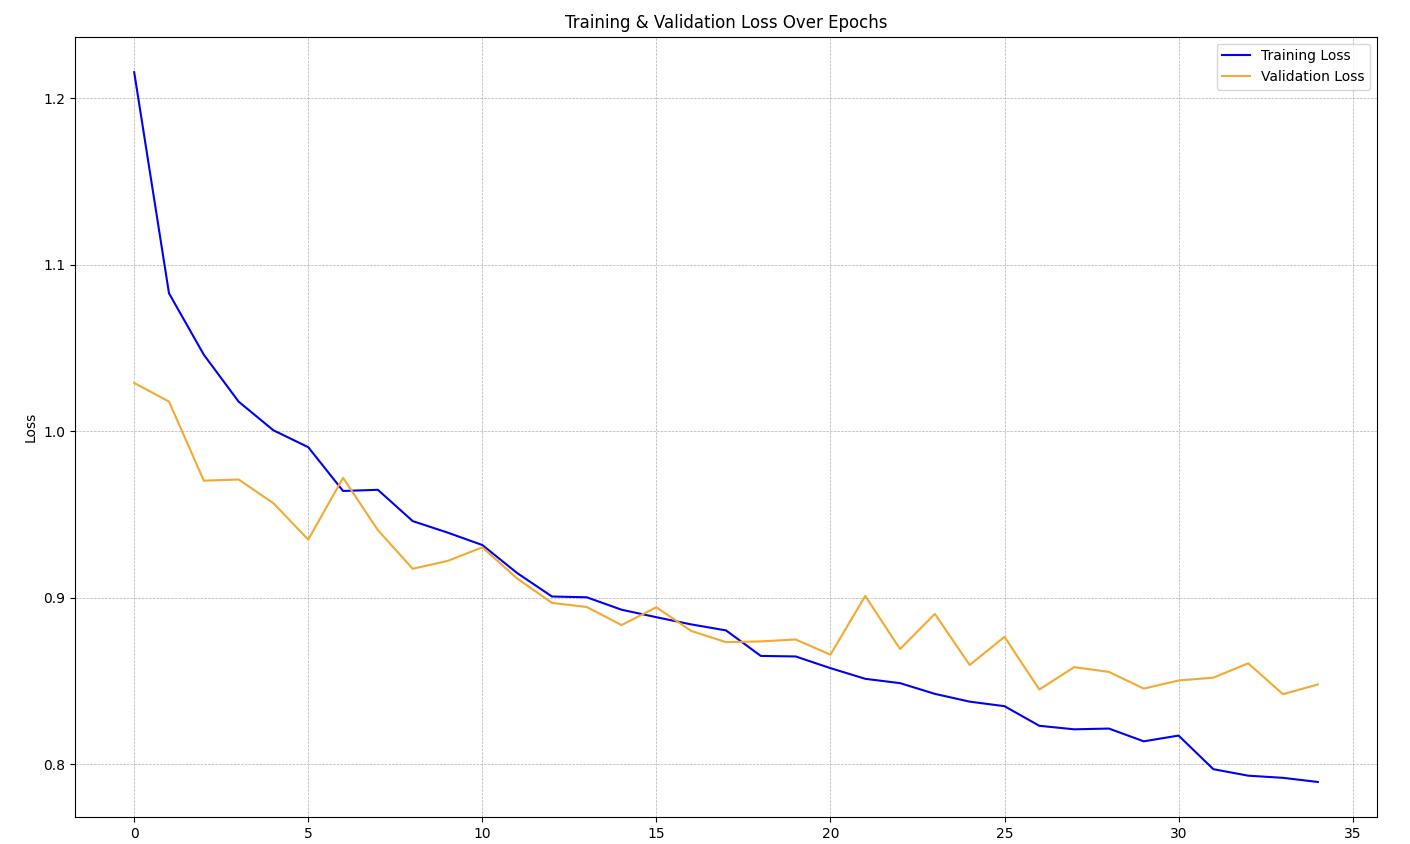
\includegraphics[width=0.8\textwidth]{images/training_loss_graph.png}
    \caption{The loss function for the final training process.}
    \label{fig:loss_graph}
\end{figure}

Training was stopped after epoch 34 to avoid overfitting on the training. The Figure~\ref{fig:loss_graph} shows the loss function on the traning and validation sets as the model trains. This model is evaluated in the quantitative and qualitative evaluation sections in Chapter~\ref{chap:results}.

\section{Mobile Application}
\label{sec:mobile_app}

To demonstrate the practical viability of the developed student model and to confirm that it meets the performance requirements on resource-constrained devices, a Proof of Concept mobile application was developed. As mentioned previously, the application was developed using the \textbf{Flutter} framework.

\subsection{Architecture}
\label{subsec:app_arch}

The application followed an architecture based on the separation of responsibilities to ensure ease of maintenance and future development. The key components are:
\begin{description}
    \item[State Management:] The \texttt{Provider} package with the \texttt{ChangeNotifier} pattern was used to manage the application's state centrally and effectively. This approach separates the business logic from the UI, where the UI listens for changes in the application state and automatically updates itself upon any change (such as selecting a new image or the completion of the processing).
    \item[Services:] The core logic was encapsulated in an isolated service layer.
    \begin{itemize}
        \item \textbf{Model Loader Service:} Responsible for loading the ONNX model from the application's assets. This service activates available Hardware Acceleration (such as NNAPI on Android and CoreML on iOS) to ensure maximum possible performance.
        \item \textbf{Depth Estimator Service:} Contains the complete logic for the depth estimation process, from image preprocessing to applying colormaps to the model's final output.
    \end{itemize}
    \item[Utils:] Helper tools required by the services.
    \item[UI (User Interface):] The UI was built from a collection of independent and reusable \texttt{Widgets}, which are then used in the display screens, making the codebase more organized and clear.
\end{description}

\subsection{Performance Optimizations}
\label{subsec:app_optimizations}

To achieve the primary performance requirement of real-time responsiveness and to avoid freezing the UI during computationally intensive operations, two main optimizations were implemented:
\begin{itemize}
    \item \textbf{Using onnxruntime:} This specialized library was relied upon for running AI models on mobile devices, as it provides the best possible performance by leveraging local hardware capabilities.
    \item \textbf{Background Processing (Isolates):} Both the image preprocessing (resizing, normalization) and the depth map post-processing (applying a colormap) are computationally intensive. To avoid blocking the main thread responsible for UI smoothness, these two operations were moved to be executed in separate background threads (\texttt{Isolates}) using the \texttt{compute} function provided by Flutter. This approach ensures the application remains fully responsive even while processing images.
\end{itemize}

\subsection{Application Features Showcase}
\label{subsec:app_features}

The application provides a simple and intuitive interface that allows the user to perform the following functions:
\begin{itemize}
    \item \textbf{Select an Image:} The user can capture a new photo using the camera or select an existing one from the gallery (See Figure~\ref{fig:app_screenshots1}).
    \item \textbf{Estimate Depth:} A dedicated button starts the depth estimation process, displaying a "Processing..." indicator to provide the user with visual feedback.
    \item \textbf{Display Results:} The original image and the resulting depth map are displayed on the same screen for immediate comparison (See Figure~\ref{fig:app_screenshots1}).
    \item \textbf{Measure Performance:} The inference time taken by the model is displayed in milliseconds below the depth map, providing a direct quantitative measure of the model's efficiency (See Figure~\ref{fig:app_screenshots1}).
    \item \textbf{Customize Display:} The user can change the colormap applied to the output (e.g., from grayscale to Viridis) to get a better visualization of the depth differences (See Figure~\ref{fig:app_screenshots2}).
    \item \textbf{Live Depth Camera:} A live camera feature provides real-time depth estimation at approximately \textbf{4 frames per second} (See Figure~\ref{fig:app_screenshots2}).
    \item \textbf{Night Mode:} The application also includes support for a dark/night mode (See Figure~\ref{fig:app_screenshots2}).
\end{itemize}

\begin{figure}[htbp!]
    \centering
    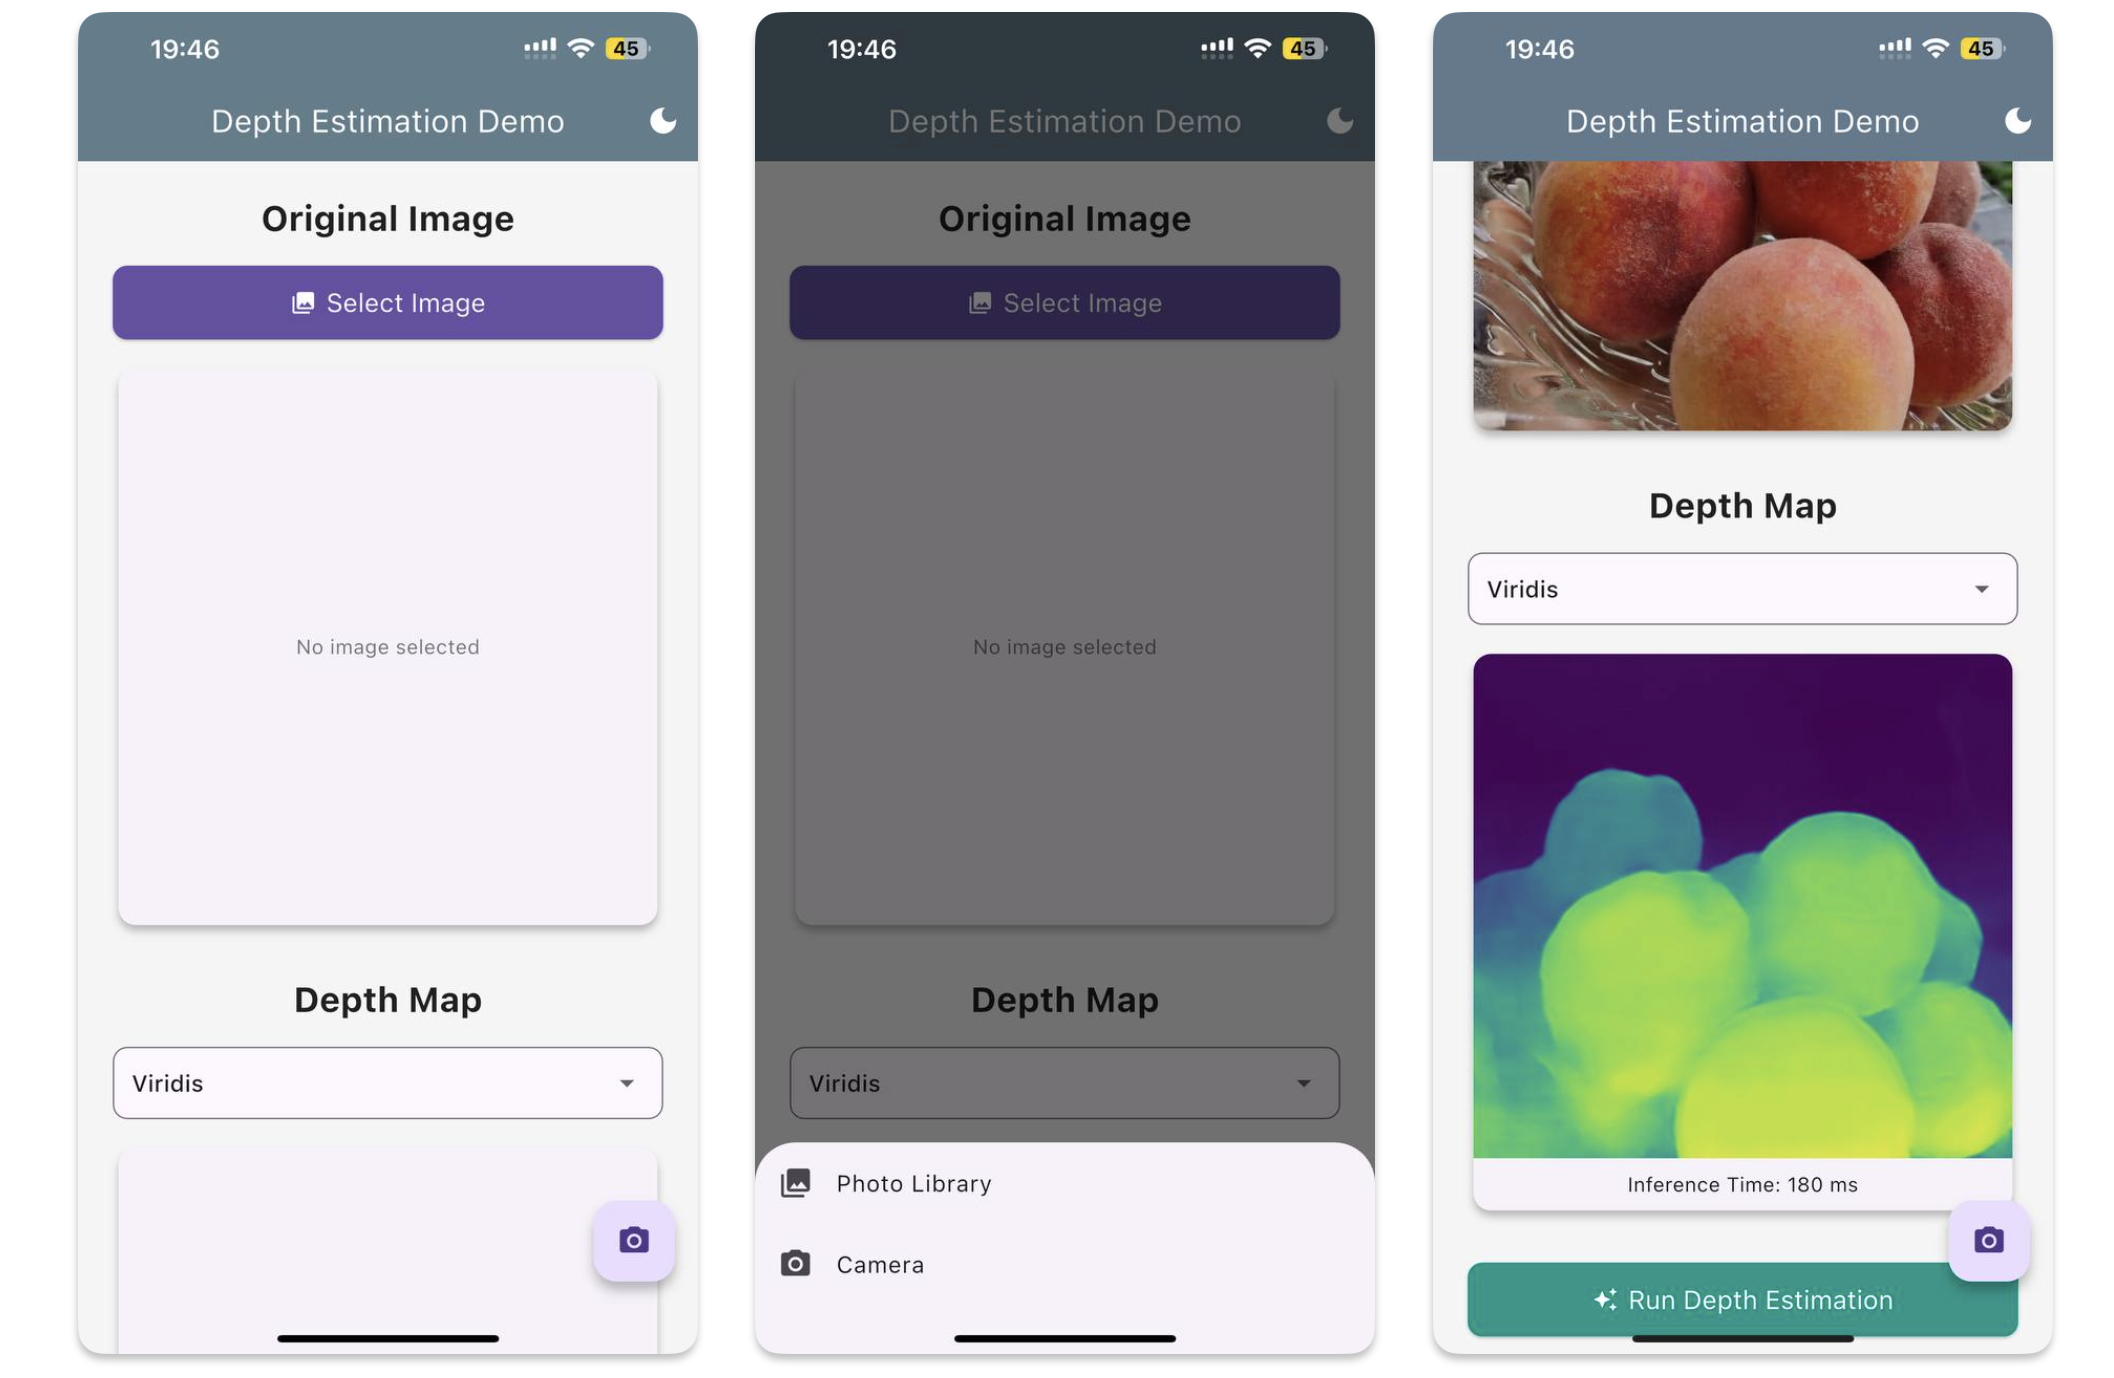
\includegraphics[width=0.9\textwidth]{images/app_screenshots_1.png}
    \caption{Image selection and result display.}
    \label{fig:app_screenshots1}
\end{figure}

\begin{figure}[htbp!]
    \centering
    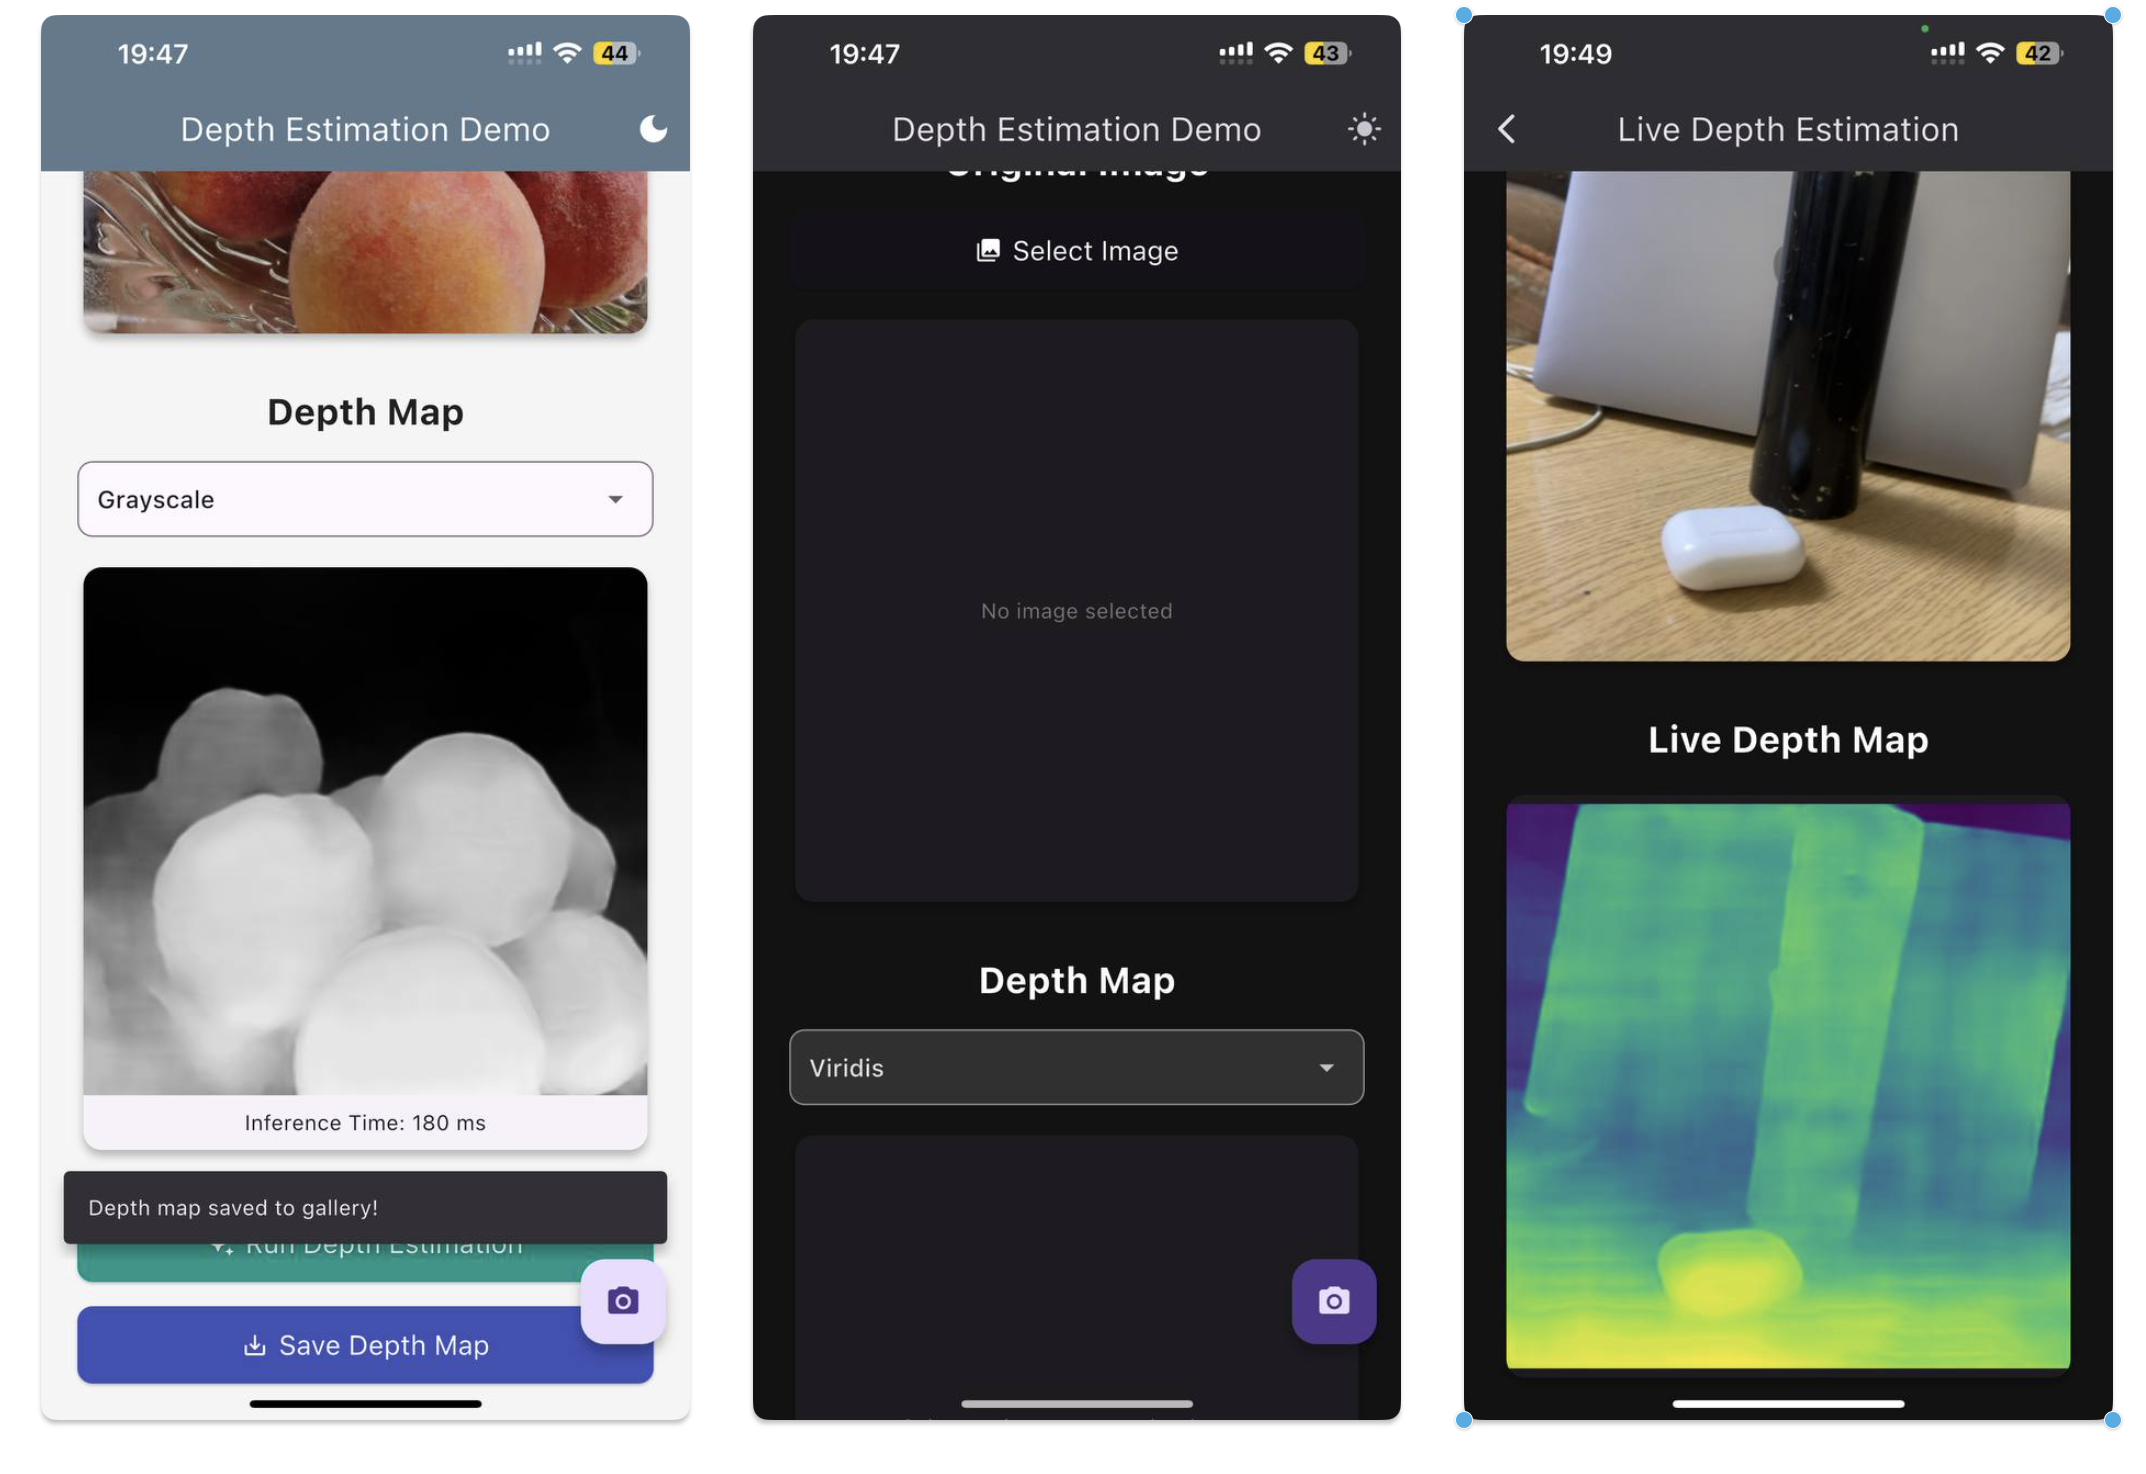
\includegraphics[width=0.9\textwidth]{images/app_screenshots_2.png}
    \caption{Live depth camera, saving the depth map, and depth visualization.}
    \label{fig:app_screenshots2}
\end{figure}

As Shown in Figure~\ref{fig:app_screenshots1} the inference time does not exceed 200 ms, which was one of our goals. Thus, the application successfully proves the effectiveness of the distilled model and its capability to run efficiently in a real-world runtime environment on mobile phones, achieving the specified goals and requirements.
% --- CHAPTER 5 ---
\chapter{Results and Discussion}
\label{chap:results}

\section{Testing Environment}
\label{sec:test_env}

The model was evaluated on the following hardware:
\begin{itemize}
    \item \textbf{Mobile Phone:} iPhone 13 (A15 processor).
    \item \textbf{Laptop:} Macbook Pro 2018 (Intel Core i7 processor).
    \item \textbf{Cloud Environment:} Google Colab (Tesla T4 GPU).
\end{itemize}

\section{Quantitative Evaluation}
\label{sec:quantitative_eval}

The final student model's performance was evaluated on a test set from NYU Depth V2 consisting of 400 images, and it was compared against the teacher model.
The Table~\ref{tab:quantitative_results} shows the achieved results using the metrics defined previously in Section~\ref{sec:evaluation_metrics}.

\begin{table}[htbp!]
    \centering
    \caption{Quantitative Evaluation of the Student Model.}
    \label{tab:quantitative_results}
    \resizebox{\textwidth}{!}{%
        \begin{tabular}{lccccccc}
            \toprule
            \textbf{Model} & \textbf{Abs Rel ($\downarrow$)} & \textbf{Sq Rel ($\downarrow$)} & \textbf{RMSE ($\downarrow$)} & \textbf{RMSE Log ($\downarrow$)} & \textbf{$\delta < 1.25$ ($\uparrow$)} & \textbf{$\delta < 1.25^2$ ($\uparrow$)} & \textbf{$\delta < 1.25^3$ ($\uparrow$)} \\
            \midrule
            Teacher & 0.2853 & 0.6857 & 1.4286 & 0.3273 & 0.6236 & 0.8340 & 0.9247 \\
            Student & 0.4068 & 0.9911 & 1.6713 & 0.3877 & 0.5733 & 0.8261 & 0.8911 \\
            \bottomrule
        \end{tabular}%
    }
\end{table}

\section{Qualitative Evaluation}
\label{sec:qualitative_eval}

The model was tested on various images. The Figure~\ref{fig:qualitative_comp} shows a comparison between the original image (left), the depth map from the teacher (middle), and the depth map from the student (right).

\begin{figure}[htbp!]
    \centering
    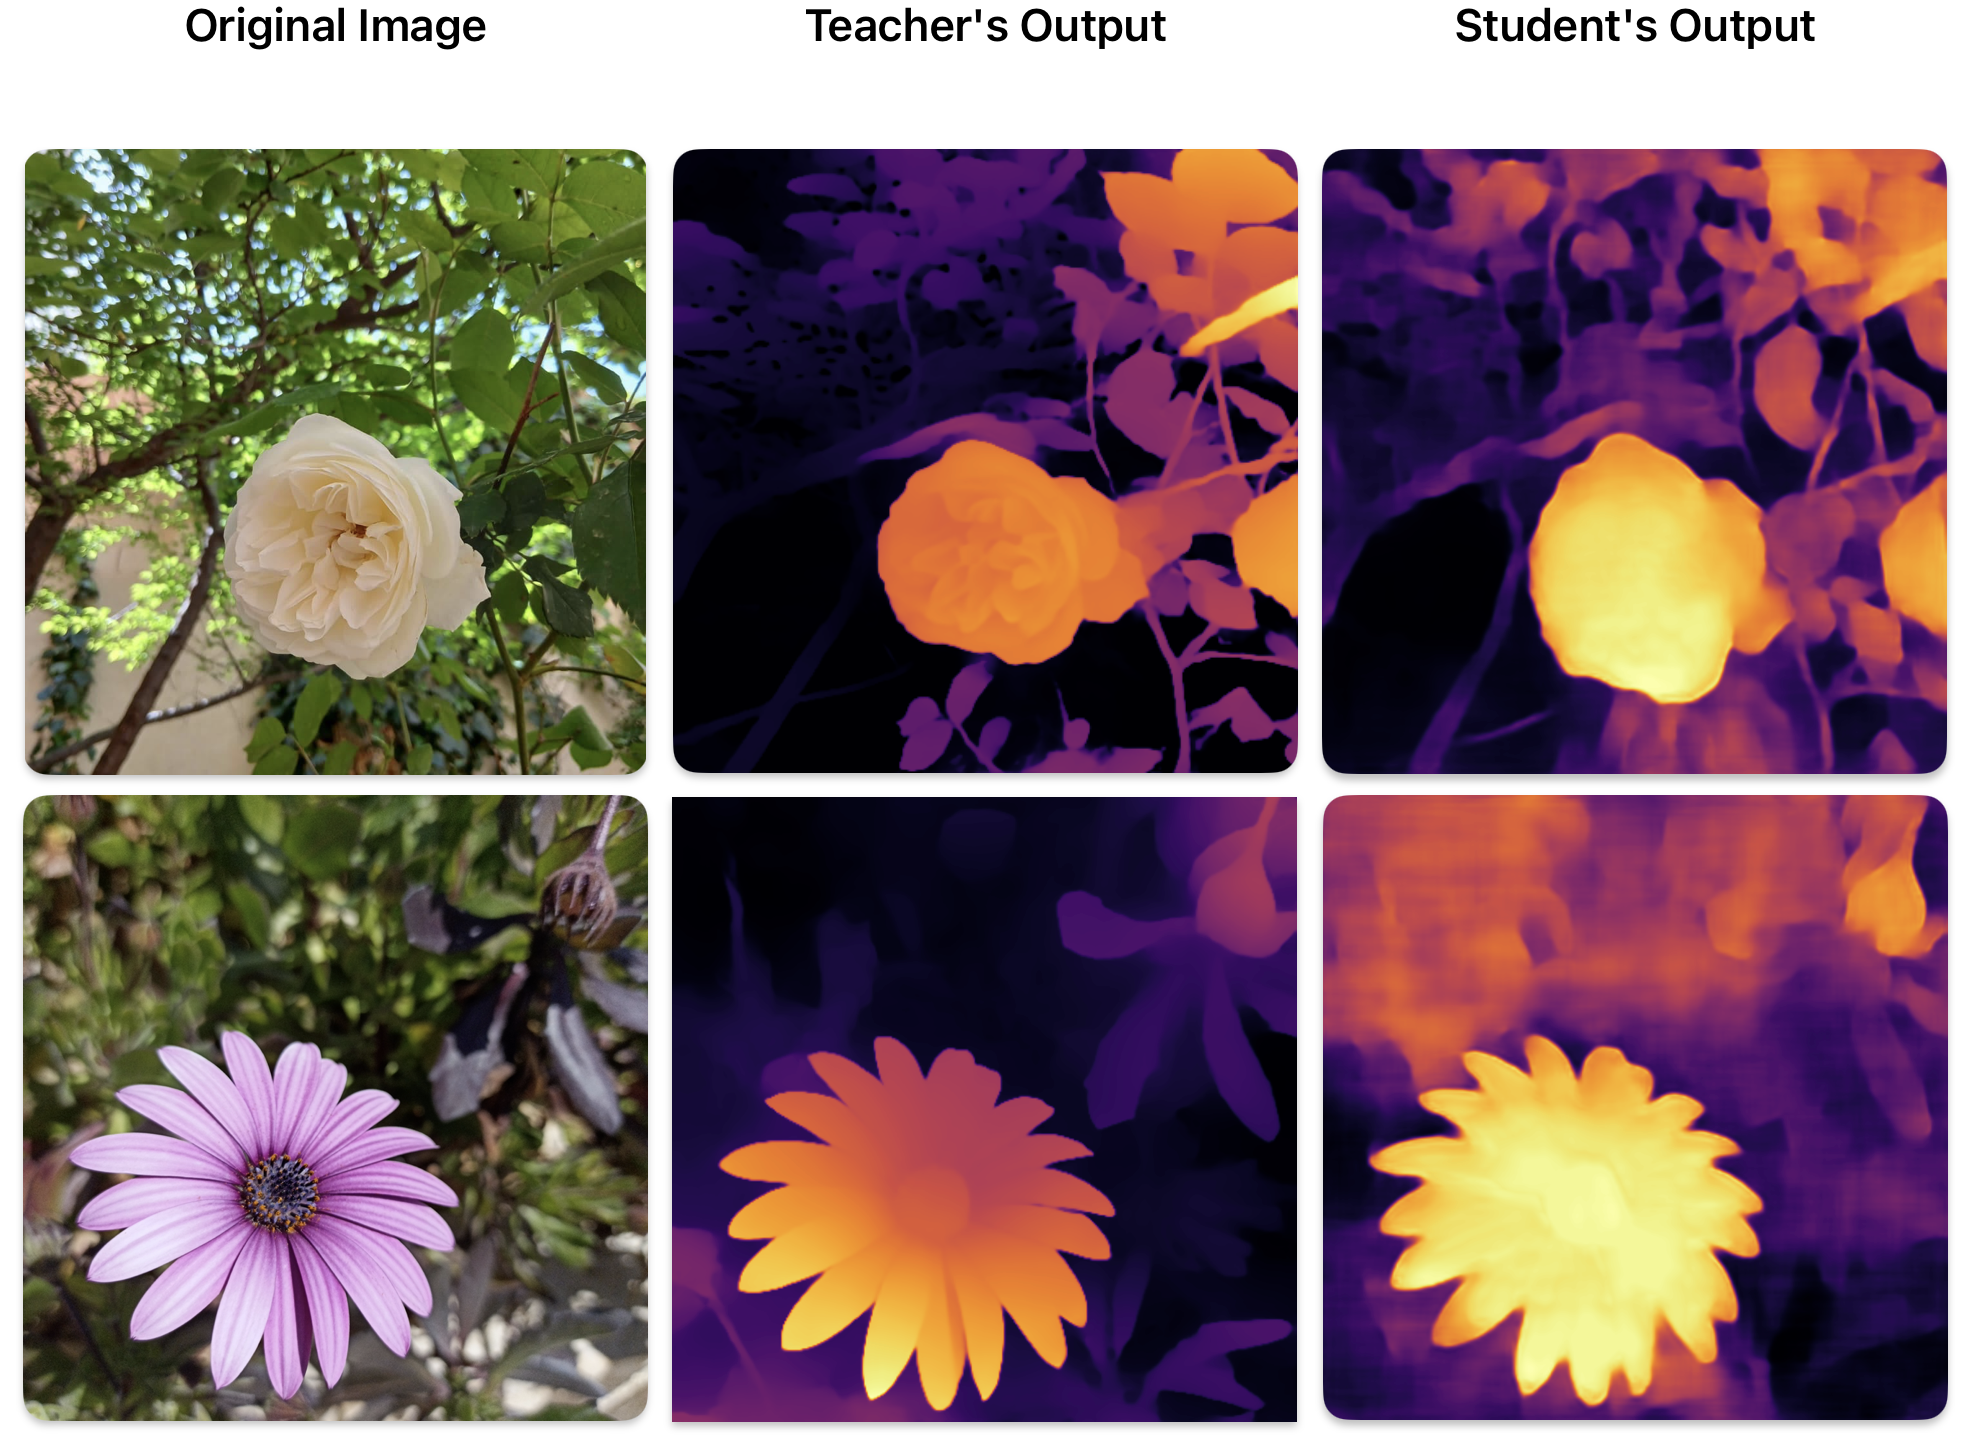
\includegraphics[width=\textwidth]{images/qualitative_comparison.png}
    \caption{Visual Comparison.}
    \label{fig:qualitative_comp}
\end{figure}

\section{Performance Measurements}
\label{sec:performance}

Performance was measured on the devices mentioned in the testing environment, and the results were as shown in Table~\ref{tab:performance}.

\begin{table}[htbp!]
    \centering
    \caption{Performance Measurements for the Model.}
    \label{tab:performance}
    \begin{tabular}{lc}
        \toprule
        \textbf{Model} & \textbf{Time (milliseconds)} \\
        \midrule
        Teacher on Laptop & $1124 \pm 10$ \\
        Student on Laptop & $576.8 \pm 10$ \\
        Teacher on Google Colab & $60 \pm 7$ \\
        Student on Google Colab & $13.2 \pm 3$ \\
        Teacher on Mobile Phone & $10751 \pm 50$ \\
        Student on Mobile Phone & $186 \pm 10$ \\
        \bottomrule
    \end{tabular}
\end{table}

We achieved an average time of 186 milliseconds on the mobile phone, which means we have achieved the desired goal.

\section{Discussion}
\label{sec:discussion}

This project has succeeded in achieving its primary objective: to demonstrate the effectiveness of knowledge distillation as a strategy for developing highly efficient depth estimation models suitable for mobile devices. The results show that the developed student model is capable of operating in near real-time within a resource-constrained environment, thus achieving the difficult balance between computational accuracy and performance requirements. Achieving an average inference time of about 186 milliseconds on a mobile phone meets the non-functional requirement of not exceeding 200 milliseconds and confirms the success of the adopted approach.

When analyzing the results, we note an expected gap in accuracy between the teacher and student models, as shown by the quantitative evaluation on the NYU Depth V2 dataset. It is worth noting that the performance of the teacher model, according to its developers, is better than what was measured here (0.05 for AbsRel~\cite{yang2024depthV2}), which indicates a bias in the dataset used for evaluation. Therefore, we focus on the gap between the student and teacher rather than the absolute value of the metrics. While this accuracy gap makes the model unsuitable for applications requiring high precision, it is well-suited for fields that tolerate a larger margin of error, such as navigation assistance. This decrease in accuracy represents a deliberate and acceptable trade-off in exchange for obtaining massive gains in performance.

The model size was reduced by a ratio of approximately 1/7 compared to the teacher. More importantly, it is now possible to run it on a mobile device with near real-time performance, which was not possible with the teacher model. Qualitative comparisons show that the student model successfully captures the general structure of the scene and the fundamental depth gradients, despite losing some of the fine details that the teacher model retains. This quality is considered sufficient for many practical applications, such as augmented reality and basic navigation aids.

The success of the model can be attributed to several deliberate methodological decisions. The choice of the MobileViT-XS architecture as the encoder was a crucial decision, as it proved its ability to understand the global context of the image, overcoming the limitations of the MobileNetV3 architecture observed in initial attempts. Furthermore, the composite loss function played a pivotal role in the distillation process: by compelling the student to mimic not only the final output but also the teacher's intermediate gradients and feature maps, a more comprehensive set of knowledge was transferred, which helped maintain the quality of the results despite the model's smaller size.

However, the project is not without limitations. Challenges that could be addressed in future work include improving depth estimation for transparent or reflective surfaces, which are known to be difficult for monocular depth models. Additionally, the model's performance in low-light conditions could be addressed by performing image pre-processing (e.g., increasing contrast).

\section{Future Work}
\label{sec:future_work}

Based on this discussion, several promising avenues for future work can be identified:
\begin{itemize}
    \item \textbf{Improve Training Data:} The most important next step is to retrain the model on more diverse public datasets like NYU Depth V2 to enhance its generalization capabilities and reduce the impact of biases in the current data.
    \item \textbf{Improve Evaluation Data:} To obtain logical and fair values for the metrics mentioned in the reference study.
    \item \textbf{Multi-stage Distillation:} This involves training a model with a number of parameters closer to the teacher (e.g., 15 million), then using it as a teacher for a smaller model, and finally using the latter as a teacher for the student model designed in this project.
    \item \textbf{Additional Architectural Improvements:} Other hybrid architectures could be explored, or the MiniDPT decoder structure could be improved to reduce the accuracy gap with the teacher without a significant increase in computational cost.
    \item \textbf{Model Quantization:} As a final optimization step, quantization techniques (such as converting weights to 16-bit or 8-bit integers) can be applied to the final ONNX model. This procedure would further reduce the model's size and accelerate inference time on supported mobile devices.
\end{itemize}


%---------- REF PAGE ----------
\newpage

\bibliographystyle{ieeetr}

\bibliography{references}



\end{document}